
\chapter{Runtime System Improvements}
\label{chap:rts}

\status{This chapter is finished!}

Early in the project
we tested two manually parallelised programs:
a raytracer and a mandelbrot image generator.
Both programs have a single significant loop
whose iterations are independent of one another.
We expect that a good automatic parallelisation system will parallelise this
loop as it is the best place to introduce parallelism.
When we parallelised this loop manually,
we did not get the speedups that we expected.
Therefore,
we chose to address the performance problems
before we worked on automatic parallelism.
Throughout this chapter
we continue to use these two benchmarks, along with a naive Fibonacci
program (Page~\pageref{page:fibs}).
These benchmarks are not diverse and they all create a lot of
AND-parallelism,
most of which is independent.
We use these benchmarks deliberately to test that our runtime system can
handle large amounts of parallelism efficiently.

In this chapter we investigate and correct these performance problems.
We start with the garbage collector in Section~\ref{sec:rts_gc};
we analyse the collector's effects on performance and tune its parameters
to improve performance.
In Section~\ref{sec:rts_original_scheduling} we describe how the existing runtime
system schedules sparks,
and provide background material for
Section~\ref{sec:rts_original_scheduling_performance},
which benchmarks the runtime system and describes two significant problems with
spark scheduling.
We address one of these problems by introducing work stealing in
Section~\ref{sec:rts_work_stealing}.
Then in Section~\ref{sec:rts_reorder} we reorder conjuncts in independent
parallel conjunctions to work around the second spark scheduling problem.
Finally, in Section~\ref{sec:rts_work_stealing2} we make further
improvements to
work stealing and change the data structures and algorithms used to manage
idle engines,
including how idle engines look for work, sleep and are woken up.


\section{Garbage Collector Tweaks}
\label{sec:gc}

One of the sources of poor parallel performance is the behaviour of the
garbage collector.
Like other pure declarative languages,
Mercury does not allow destructive update.
%\footnote{
%    Destructive update is allowed via support for mutable variables.
%    Their use does not interfere with parallelism as they are used in
%    conjunction with impurity.
%    The compiler will not parallelise impure goals.}
Therefore a call usually returns its value in newly allocated memory
rather than modifying the memory of its parameters.
Likewise, a call cannot modify global memory.
This means that Mercury programs often have a high rate of allocation,
which places significant stress on the garbage collector.
Therefore,
allocation and garbage collection can reduce a program's
performance.
This usually becomes more significant when parallelism is introduced into a
program.

\plan{Introduce Boehm, \& details: conservative, mark and sweep, stop the
world, parallel marking.}
Mercury uses the Boehm-Demers-Weiser conservative garbage collector (Boehm GC)
\citep{boehm:1988:gc},
which is a conservative mark and sweep collector.
Boehm GC supports parallel programming:
it will stop all the program's threads (\emph{stop the world}) during its
marking phase.
It also supports parallel marking:
it will use its own set of pthreads to do parallel marking.

\plan{Introduce collector time, mutator time.}
For the purposes of this section
we separate the program's execution time into two alternating phases:
Collection time, which is when Boehm GC performs marking,
and mutator time, which is when the Mercury program runs.
The name `mutator time' refers to time that mutations (changes) to memory
structures are permitted.
The collector may also perform some actions,
such as sweeping,
concurrently with the mutator.

\plan{Describe theory of GC performance.}
Amdahl's law~\citep{amdahl:1967:law} describes the maximum speedup that
can theoretically be achieved by parallelising a part of a program.
We use Amdahl's law to predict the speedup of a program whose
mutator is parallelised but whose collector runs sequentially.
Consider a program with a runtime of 20 seconds
which can be separated into one second of collector time and 19 seconds
of mutator time.
The sequential execution time of the program is $1 + 19 = 20$.
If we parallelise the mutator and do not parallelise the
collector then the minimum parallel execution time is $1 + 19/P$
for $P$ processors.
Using four processors the theoretical best speedup is:
%\paul{I prefer how \\frac displays maths but in text the fonts become tiny.}
$(1 + 19) / (1 + 19/4) = 3.48$.
17\% of the parallel runtime ($1 + 19/4$) is collector time.
If we use a machine with 100 processors then this becomes:
$(1 + 19) / (1 + 19/100) = 16.8$;
with 84\% of the runtime spent in the collector.
As the number of processors increases,
the mutator threads spend a larger proportion of their time waiting for
collection to complete.

\plan{Discuss predictions regarding parallel marking, locking and thread
local heaps.}
To reduce this problem,
\citet{boehm:1988:gc} included parallel marking support in their collector.
Ideally this would remove the bottleneck described above.
However,
parallel garbage collection is a continuing area of research and
the Boehm GC project has only modest multicore scalability goals.
Therefore,
we expect parallel marking to only partially reduce the bottleneck,
rather than remove it completely.

Furthermore, thread safety has two significant performance costs;
These types of costs prevent us from achieving the theoretical maximum
speedups that Amdahl's law predicts.
The first of these is that
one less CPU register is available to GCC's code generator when compiling
parallel Mercury programs (section \ref{sec:backgnd_merpar}).
The second is that
memory allocation routines must use locking to protect shared data
structures,
which will slow down allocation.
Boehm GC's authors recognised this problem and
added support for thread-local resources such as free lists.
Therefore,
during memory allocation,
a thread uses its own free lists rather than locking a global structure.
From time to time, a thread will have to retrieve new free lists
from a global structure and will need to lock the structure.
The costs of locking will be amortised across several memory allocations.

\plan{Describe icfp2000, mandelbrot\_lowalloc and mandelbrot\_highalloc
programs.}
To how well Mercury and Boehm GC scale to multiple cores we used several
benchmark programs with different memory allocation requirements.
Our first benchmark is a raytracer developed for the
ICFP programming contest in 2000.
For each pixel in the image,
the raytracer casts a ray into the scene to determine what colour to paint that pixel.
Two nested loops build the pixels for the image:
the outer loop iterates over the rows in the image and
the inner loop iterates over the pixels in each row.
We manually parallelised the program by introducing an parallel
conjunction into the outer loop;
indicating that rows should be drawn in parallel.
This parallelisation is independent.
The raytracer uses many small structures to represent vectors and a pixel's
colour.
It is therefore memory allocation intensive.
Since we suspected that garbage collection was having a negative affect on
performance,
we developed a mandelbrot image generator.
The mandelbrot image generator has a similar structure to the raytracer:
it draws an image using two nested loops as above.
The mandelbrot image is drawn on the complex number plane.
A complex number $C$ is in the mandelbrot set if
$\forall i \cdot |N_i| < 2$ where $N_0 = 0$ and $N_{i+1} = N_{i}^2 + C$.
For each pixel in the image the program tests if the pixel's coordinates are
in the set.
The pixel's colour is chosen based on how many iterations $i$ are needed
before $|N_i| \ge 2$,
or black if the test survived 5,000 iterations.
We parallelised this program the same way as we did the raytracer:
by introducing an independent parallel conjunction into the outer loop.
We created two versions of this program.
The first version represents coordinates and complex numbers as structures
on the heap.
Therefore it has a high rate of memory allocation.
We call this version `mandelbrot\_highalloc'.
The second version of the mandelbrot program,
called `mandelbrot\_lowalloc',
stores its coordinates and complex numbers on the stack and in registers.
Therefore it has a lower rate of memory allocation.


\begin{table}
\begin{center}
\begin{tabular}{r|rr|rrrr}
\Cbr{GC Markers} &
\multicolumn{2}{c|}{Sequential} &
\multicolumn{4}{c}{Parallel w/ $N$ Mercury Engines} \\
\Cbr{} &
\C{no TS} & \Cbr{TS} &
\C{1} & \C{2} & \C{3} & \C{4} \\
\hline
\hline
\multicolumn{7}{c}{raytracer} \\
\hline
1 & 33.1 (1.13) & 37.4 (1.00) &
             37.7 (0.99) & 28.0 (1.34) & 24.8 (1.51) & 23.7 (1.58) \\
2  & - & - & 32.0 (1.17) & 21.6 (1.73) & 18.1 (2.07) & 16.7 (2.24) \\
3  & - & - & 29.6 (1.26) & 19.7 (1.90) & 16.3 (2.29) & 14.5 (2.59) \\
4  & - & - & 29.1 (1.29) & 18.9 (1.98) & 15.3 (2.45) & 13.7 (2.73) \\
\hline
\hline
\multicolumn{7}{c}{mandelbrot\_highalloc} \\
\hline
1 & 41.0 (1.23) & 50.5 (1.00) &
             50.6 (1.00) & 33.4 (1.51) & 26.6 (1.90) & 23.4 (2.16) \\
2  & - & - & 46.7 (1.08) & 28.6 (1.77) & 22.1 (2.28) & 18.8 (2.69) \\
3  & - & - & 46.3 (1.09) & 27.3 (1.85) & 20.9 (2.42) & 17.3 (2.93) \\
4  & - & - & 45.6 (1.11) & 26.8 (1.89) & 20.4 (2.48) & 16.7 (3.03) \\
\hline
\hline
\multicolumn{7}{c}{mandelbrot\_lowalloc} \\
\hline
1 & 15.4 (0.99) & 15.2 (1.00) &
             15.2 (1.00) &  5.1 (2.96) &  7.7 (1.98) &  3.9 (3.92) \\
2  & - & - & 15.3 (1.00) &  7.7 (1.98) &  5.1 (2.97) &  3.9 (3.94) \\
3  & - & - & 14.3 (1.00) &  7.7 (1.98) &  5.1 (2.97) &  3.9 (3.94) \\
4  & - & - & 15.3 (0.99) &  7.7 (1.98) &  5.1 (2.97) &  3.9 (3.92) \\ 
\end{tabular}
\end{center}
\paul{Consider drawing charts for raytracer and mandelbrot so that releative
performance between different scores can be seen easily.}
\caption{Parallelism and garbage collection}
\label{tab:gc}
\end{table}



\plan{Benchmark data.}
We benchmarked these three programs with different numbers of Mercury
engines and garbage collector threads.
We show the results in table \ref{tab:gc}.
All benchmarks have an initial heap size of 16MB.
Each result is measured in seconds and represents the mean of eight samples.
The first column is the number of garbage collector threads used.
The second and third columns give sequential execution times
without and with thread safety enabled.
In these columns the programs where executed in such a way so that they did
not execute a parallel conjunction.
The remaining four columns give parallel execution times using one to four
Mercury engines.
The numbers in parentheses show the relative speedup when compared with the
sequential thread safe result for the same program.
\label{cabsav}
We ran our benchmarks on
\paul{Find a brand name i7 I can borrow for some weeks}
a Intel i7-2600K system
with 16GB of memory,
running Debian/GNU Linux 6
with a 2.6.32-5-amd64 Linux kernel and GCC 4.4.5-8.
The garbage collection benchmarks were gathered using a recent version of
Mercury (rotd-2012-04-29).
This version does not have the performance problems described in the
rest of this chapter,
and it does have the loop control transformation described
in chapter \ref{chap:loop_control}.
Therefore we can observe the effects of garbage collection without
interference from any other performance problems.

\plan{Describe performance in practice.}
The raytracer program benefits from parallelism in both Mercury and the
garbage collector.
Using Mercury's parallelism only (four Mercury engines, and one GC thread) 
speeds the program up by a factor of 1.58,
compared to 1.29 when using the GC's parallelism only (one Mercury engine,
and four GC threads).
When using both Mercury and the GC's parallelism (four engines and four
marker threads)
the raytracer achieves a speedup of 2.73.
These speedups are much lower than we might expect from such a program:
either the mutator, the collector or both are not being parallelised well.
mandelbrot\_lowalloc does not see any benefit from parallel marking.
It achieves very good speedups from multiple Mercury engines.
We know that this program has a low allocation rate
but is otherwise parallelised in the same way as raytracer.
Therefore,
these results support the hypothesis that heavy use of garbage collection
makes it difficult to achieve good speedups when parallelising programs.
The more time spend in garbage collection,
the worse the speedup due to parallelism.
mandelbrot\_highalloc, which stores its data on the heap,
sees similar trends in performance as raytracer.
It is also universally slower than mandelbrot\_lowalloc.
mandelbrot\_highalloc achieves a speedup of 2.16 when using parallelism in
Mercury (four Mercury engines, and one GC thread).
The corresponding figure for the raytracer is 1.58.
When using the GC's parallelism
(one Mercury engine, and four GC threads)
mandelbrot\_highalloc achieves a speedup of 1.11,
compared with 1.29 for the raytracer.


\begin{table}
\begin{center}
\begin{tabular}{r|l| d{1} r | d{1} r | d{1} r | d{1} r }
\C{GC} & \C{Times \&} &
\multicolumn{8}{c}{Parallel w/ $N$ Mercury Engines} \\
\C{Markers} & \C{Collections}
          & \Ctwo{1}        & \Ctwo{2}        & \Ctwo{3}        & \Ctwo{4} \\
\hline
\hline
\multicolumn{10}{c}{raytracer} \\
\hline
\multirow{4}{*}{1} &
  Elapsed & 37.8 &        & 28.1 &        & 24.7 &        & 22.7 & \\
& GC      & 16.9 & 44.8\% & 16.7 & 59.4\% & 16.5 & 66.6\% & 15.8 & 69.5\% \\
& Mutator & 20.9 & 55.2\% & 11.4 & 40.6\% &  8.2 & 33.4\% &  6.9 & 30.5\% \\
& \# col. & 384. &        &346.  &        &316.  &        &288.  & \\
\hline
\multirow{4}{*}{2} &
  Elapsed & 32.6 &        & 21.8 &        & 18.3 &        & 16.0 & \\
& GC      & 11.0 & 33.8\% & 10.4 & 47.7\% & 10.3 & 56.4\% &  9.8 & 60.8\% \\
& Mutator & 21.6 & 66.2\% & 11.4 & 52.3\& &  8.0 & 43.6\% &  6.3 & 39.2\% \\
& \# col. & 384. &        &346.  &        &316.  &        &288.  & \\
\hline
\multirow{4}{*}{3} &
  Elapsed & 30.9 &        & 20.0 &        & 16.4 &        & 14.1 & \\
& GC      &  9.3 & 30.2\% &  8.5 & 42.3\% &  8.2 & 50.0\% &  7.8 & 55.4\% \\
& Mutator & 21.6 & 69.8\% & 11.5 & 57.7\% &  8.2 & 50.0\% &  6.3 & 44.6\% \\
& \# col. & 386. &        &346.  &        &316.  &        &288.  & \\
\hline
\multirow{4}{*}{4} &
  Elapsed & 30.3 &        & 19.3 &        & 15.5 &        & 13.5 & \\
& GC      &  8.7 & 28.8\% &  7.8 & 40.4\% &  7.4 & 47.8\% &  7.1 & 52.4\% \\
& Mutator & 21.6 & 71.2\% & 11.5 & 59.6\% &  8.1 & 52.2\% &  6.4 & 47.6\% \\
& \# col. & 387. &        &346.  &        &316.  &        &288.  & \\
\hline
\hline
\multicolumn{10}{c}{mandelbrot\_highalloc} \\
\hline
\multirow{4}{*}{1} &
  Elapsed & 51.7 &        & 34.0 &        & 27.2 &        & 24.0 & \\
& GC      & 11.0 & 21.4\% & 11.5 & 33.6\% & 11.5 & 42.2\% & 11.8 & 49.1\% \\
& Mutator & 40.7 & 78.6\% & 22.6 & 55.4\% & 15.5 & 57.8\% & 12.2 & 50.9\% \\
& \# col. &742.  &        &692.  &        &634.  &        &602. & \\
\hline
\multirow{4}{*}{2} &
  Elapsed & 48.5 &        & 29.3 &        & 22.3 &        & 19.1 & \\
& GC      &  6.4 & 13.1\% &  6.7 & 22.9\% &  6.6 & 29.7\% &  6.9 & 36.1\% \\
& Mutator & 42.1 & 86.9\% & 22.6 & 77.1\% & 15.7 & 70.3\% & 12.2 & 63.9\% \\
& \# col. &744.  &        &693.  &        &633.  &        &595.  & \\
\hline
\multirow{4}{*}{3} &
  Elapsed & 46.4 &        & 28.0 &        & 21.0 &        & 17.7 & \\
& GC      &  5.0 & 10.8\% &  5.3 & 18.8\% &  5.3 & 25.0\% &  5.4 & 30.4\% \\
& Mutator & 41.4 & 89.2\% & 22.8 & 81.2\% & 15.7 & 75.0\% & 12.3 & 69.6\% \\
& \# col. &737.  &        &692.  &        &629.  &        &600.  & \\
\hline
\multirow{4}{*}{4} &
  Elapsed & 46.0 &        & 27.6 &        & 20.3 &        & 16.9 & \\
& GC      &  4.5 &  9.9\% &  4.7 & 17.0\% &  4.6 & 22.6\% &  4.7 & 27.6\% \\
& Mutator & 41.4 & 90.1\% & 22.9 & 83.0\% & 15.7 & 77.4\% & 12.3 & 72.4\% \\
& \# col. &740.  &        &695.  &        &626.  &        &600.  & \\
\hline
\hline
\multicolumn{10}{c}{mandelbrot\_lowalloc} \\
\hline
\multirow{4}{*}{1} &
  Elapsed & 15.2 &        &  7.7 &        &  5.1 &        &  3.9 & \\
& GC      &  0.0 &  0.1\% &  0.0 &  0.2\% &  0.0 &  0.7\% &  0.0 &  0.4\% \\
& Mutator & 15.2 & 99.9\% &  7.6 & 99.8\% &  5.1 & 99.3\% &  3.9 & 99.6\% \\
& \# col. &  2.  &        &  2.  &        &  2.  &        &  2.  & \\
\hline
\multirow{4}{*}{2} &
  Elapsed & 15.4 &        &  7.6 &        &  5.1 &        &  3.9 & \\
& GC      &  0.0 &  0.1\% &  0.0 &  0.1\% &  0.0 &  0.2\% &  0.0 &  0.2\% \\
& Mutator & 15.4 & 99.9\% &  7.6 & 99.9\% &  5.1 & 99.8\% &  3.9 & 99.8\% \\
& \# col. &  2.  &        &  2.  &        &  2.  &        &  2.  & \\
\hline
\multirow{4}{*}{3} &
  Elapsed & 15.3 &        &  7.7 &        &  5.1 &        &  3.9 & \\
& GC      &  0.0 &  0.1\% &  0.0 &  0.1\% &  0.0 &  0.4\% &  0.0 &  0.1\% \\
& Mutator & 15.2 & 99.9\% &  7.7 & 99.9\% &  5.1 & 99.6\% &  3.9 & 99.9\% \\
& \# col  &  2.  &        &  2.  &        &  2.  &        &  2.  & \\
\hline
\multirow{4}{*}{4} &
  Elapsed & 15.2 &        &  7.6 &        &  5.1 &        &  3.9 & \\
& GC      &  0.0 &  0.1\% &  0.0 &  0.1\% &  0.0 &  0.4\% &  0.0 &  0.1\% \\
& Mutator & 15.2 & 99.9\% &  7.6 & 99.9\% &  5.1 & 99.6\% &  3.9 & 99.9\% \\
& \# col  &  2.  &        &  2.  &        &  2.  &        &  2.  & \\
\end{tabular}
\end{center}
\caption{Percentage of elapsed execution time used by GC/Mutator}
\label{tab:gc_amdahl}
\end{table}



\plan{Introduce the table we use for our discussion of Amdahl's law.}
We can see that mandelbrot\_highalloc benefits from parallelism in Mercury
more than raytracer does,
conversely mandelbrot\_highalloc benefits from parallelism in the garbage
collector less than raytracer does.
Using \tscope (chapter \ref{chap:tscope}),
we analysed how much time these programs spend running the garbage collector
or the mutator.
These results are shown in table \ref{tab:gc_amdahl}.
The table shows the elapsed time, collector time, mutator time and the
number of collections for each program using one to four engines, and one
to four collector threads.
The times are averages taken from eight samples,
using an initial heap size of 16MB.
To use \tscope we had to compile the runtime system differently.
Therefore,
these results differ slightly from those in table \ref{tab:gc}.
Next to both the collector time and mutator time
we show the percentage of elapsed time taken by the collector or mutator
respectively.

\plan{Describe trends in either the mutator or GC time.}
As we expected, mandelbrot\_lowalloc spends very little time running the collector.
Typically, it ran the collector only twice during its execution.
Also, total collector time was usually between 5 and 30 milliseconds.
The other two programs ran the collector hundreds of times.
As we increased the number of Mercury engines
we noticed that these programs made fewer collections.
As we varied the number of collector threads,
we saw no trend in the number of collections.
Any apparent variation is most likely noise in the data.
All three programs see a speedup in the time spent in the mutator as the
number of Mercury engines is increased.
Similarly,
the raytracer and mandelbrot\_highalloc benefit from speedups
in GC time as the number of GC threads is increased.
In mandelbrot\_highalloc,
the GC time also increases slightly as Mercury engines are added.
We expect that as more Mercury engines are used the garbage collector
must use more inter-core communication which has additional costs.
However, in the raytracer,
the GC time decreases slightly as Mercury engines are added.
To understand why this happens we would need to understand the collector in
detail,
however Boehm GC's sources are notorious for being difficult to read and
understand.

\plan{Compare performance with Amdahl's predictions.}
As Amdahl's law predicts,
parallelism in one part of the program has a limited effect on the program
as a whole.
While using one GC thread
we tested with one to four Mercury engines;
the mutator time speedups for two, three and four engines were
1.83, 2.55 and 3.03 respectively.
However, the elapsed time speedups for the same test were only
1.35, 1.53 and 1.66 respectively.
Although there is little change in absolute time spent in the collector;
there is an increase in collector time as a percentage of elapsed time.
The corresponding mutator time speedups for mandelbrot\_highalloc were
similar,
at 1.80, 2.63 and 3.34 for two, three and four Mercury engines.
The elapsed time speedups on the same test for mandelbrot\_highalloc were
1.52, 1.90 and 2.15.
Like raytracer above, the elapsed time speedups are lower than the mutator
time speedups.
Similarly,
when we increase the number of threads used by the collector,
it improves collection time more than it does elapsed time.

When we increased both the number of threads used by the collector and the
number of Mercury engines
(a diagonal path through the table)
both the collector and mutator time decrease.
This shows that parallelism in Mercury and in Boehm GC both contribute to
the elapsed time speedup we saw in the diagonal path in table \ref{tab:gc}.
As table \ref{tab:gc_amdahl} give us more detail,
we can also see that collector time as a percentage of elapsed time
increases as we add threads and engines to the collector and Mercury.
This occurs for both the raytracer and mandelbrot\_highalloc.
It suggests that the mutator makes better use of additional Mercury
engines
than the collector makes use of additional threads.
We can confirm this by comparing the speedup for the mutator with the speedup
in the collector.
In the case of raytracer using four Mercury engines and one GC thread
the mutator's speedup is $20.9 / 6.9 = 3.03$ over the case for one Mercury
engine and one GC thread.
The collectors speedup with four GC threads and one Mercury engine over
the case for one GC thread and one Mercury engine is $16.9 / 8.7 = 1.94$.
The equivalent speedups for mandelbrot\_highalloc are:
$40.7 / 12.2 = 3.34$ and $11.0 / 4.5 = 2.44$.
Similar comparisons can be made along the diagonal of the table.

\begin{table}
\begin{center}
\begin{tabular}{l|rr|d{3}}
\Cbr{Program} & \C{Allocations} & \Cbr{Total alloc'd bytes} & \C{Alloc rate (M alloc/sec)} \\
\hline
raytracer   &     561,431,515 &           9,972,697,312 & 26.9 \\
mandelbrot\_highalloc
            &   3,829,971,662 &          29,275,209,824 & 94.1 \\
mandelbrot\_lowalloc
            &       1,620,928 &              21,598,088 &  0.106 \\
\end{tabular}
\end{center}
\caption{Memory allocation rates}
\label{tab:mem_alloc_rate}
\end{table}

\plan{Allocation intensity}
table \ref{tab:gc_amdahl} also shows that raytracer spends more of its
elapsed time doing garbage collection than mandelbrot\_highalloc does.
This matches the results in table \ref{tab:gc},
where mandelbrot\_highalloc has better speedups because of parallelism in
Mercury than raytracer does.
Likewise,
raytracer has better speedups because of parallelism in the collector
than mandelbrot\_highalloc does.
This suggests that mandelbrot\_highalloc is less allocation intensive than
raytracer,
but this is not true.
Using Mercury's deep profiler we measured the number and total size of memory
allocations.
This is shown in table \ref{tab:mem_alloc_rate}.
The rightmost column in this table gives the allocation rate
measured in million allocations per second.
It is calculated by dividing the number of allocations in the second column
by the average mutator time reported in table \ref{tab:gc_amdahl}.
Therefore, it represents the allocation rate during mutation time.
This is deliberate because,
by definition,
allocation cannot occur during collector time.
mandelbrot\_highalloc has a higher allocation rate than raytracer.
However,
it spends less time doing collection, when measured either absolutely
or by percentage of elapsed time.
Garbage collectors are tuned for particular workloads.
It is likely that Boehm GC handles mandelbrot\_highalloc's workload more
easily than raytracer's workload.

% Old idea:
%This may be due to changing allocation rates throughout the programs'
%executions.
%We noticed that while benchmarking the raytracer that if we rendered the
%image upside-down (by iterating over the rows backwards)
%we would get different performance results.
%This is because the top of the image we used contains sky,
%which has no geometry;
%it is the flat colour of the background,
%and the bottom of the image contains ground;
%which has more detail.
%Rendering the ground will naturally be more complicated and require more
%memory allocation than rendering the sky.
%Memory allocation in one part of a program can affect the performance of
%allocation and collection in another part of the program.
%This is many because the garbage collector will increase the size of the heap
%to satisfy large and/or many allocations.
%This is why rendering the image upside down had a different execution time to
%rendering it the right way up.
%Similarly,
%the mandelbrot program has sections in its image that require more iterations
%of the equation than others.


\begin{table}
\begin{center}
\begin{tabular}{r|rr|rrrr}
\Cbr{Initial} &
\multicolumn{2}{c|}{Sequential} &
\multicolumn{4}{c}{Parallel w/ $N$ Mercury Engines} \\
\Cbr{heap size} & \C{no TS}   & \Cbr{TS}    & \C{1}       & \C{2}       & \C{3}       & \C{4} \\
\hline
\hline
\multicolumn{7}{c}{raytracer} \\
\hline
1MB     & 32.8 (0.89) & 29.3 (1.00) & 29.3 (1.00) & 19.0 (1.54) & 15.4 (1.90) & 13.6 (2.16) \\
16MB    & 33.5 (0.89) & 29.7 (1.00) & 29.1 (1.02) & 18.9 (1.57) & 15.3 (1.94) & 13.7 (2.17) \\
32MB    & 34.3 (0.86) & 29.5 (1.00) & 29.5 (1.00) & 19.5 (1.51) & 15.6 (1.89) & 13.6 (2.16) \\
64MB    & 33.2 (0.92) & 30.4 (1.00) & 30.7 (0.99) & 20.3 (1.50) & 16.4 (1.86) & 14.5 (2.10) \\
128MB   & 22.7 (1.08) & 24.5 (1.00) & 24.2 (1.01) & 15.0 (1.63) & 11.7 (2.09) & 10.2 (2.40) \\
256MB   & 18.8 (1.13) & 21.4 (1.00) & 21.5 (0.99) & 12.6 (1.70) &  9.3 (2.29) &  7.7 (2.76) \\
384MB   & 17.7 (1.17) & 20.8 (1.00) & 20.7 (1.01) & 11.7 (1.77) &  8.7 (2.39) &  7.2 (2.90) \\
512MB   & 17.3 (1.17) & 20.3 (1.00) & 20.5 (0.99) & 11.5 (1.77) &  8.3 (2.44) &  6.8 (2.99) \\
\hline
\hline
\multicolumn{7}{c}{mandelbrot\_highalloc} \\
\hline
1MB     & 41.4 (1.10) & 45.5 (1.00) & 45.1 (1.01) & 26.7 (1.70) & 20.3 (2.24) & 16.7 (2.72) \\ 
16MB    & 39.7 (1.14) & 45.3 (1.00) & 45.6 (0.99) & 26.8 (1.69) & 20.4 (2.23) & 16.7 (2.72) \\
32MB    & 38.9 (1.16) & 45.2 (1.00) & 44.2 (1.02) & 26.3 (1.72) & 19.7 (2.29) & 16.5 (2.74) \\
64MB    & 36.7 (1.21) & 44.4 (1.00) & 43.7 (1.02) & 25.2 (1.76) & 18.8 (2.36) & 15.6 (2.84) \\
128MB   & 34.1 (1.25) & 42.6 (1.00) & 41.8 (1.02) & 24.1 (1.77) & 17.7 (2.41) & 14.4 (2.96) \\
256MB   & 33.2 (1.24) & 41.3 (1.00) & 41.9 (0.99) & 23.7 (1.74) & 16.9 (2.45) & 13.6 (3.04) \\ 
384MB   & 31.7 (1.29) & 41.0 (1.00) & 41.9 (0.98) & 23.3 (1.76) & 16.7 (2.46) & 13.4 (3.07) \\
512MB   & 31.1 (1.32) & 41.1 (1.00) & 41.1 (1.00) & 23.0 (1.79) & 16.7 (2.46) & 13.3 (3.08) \\ 
\end{tabular}
\end{center}
\caption{Varying the initial heapsize in parallel Mercury programs.}
\label{tab:heapsize}
\end{table}



\plan{New data, vary the heap size.}
So far,
we have shown that speedups due to Mercury's parallel conjunction
are limited by the garbage collector.
Better speedups can be achieved by using the parallel marking feature in the
garbage collector.
We also attempted to improve performance further by modifying the initial
heap size of the program.
table \ref{tab:gc_heapsize} shows the performance of the raytracer and
mandelbrot\_highalloc programs with various initial heap sizes.
The first column shows the heap size used;
we picked a number of sizes from 1MB to 512MB.
The remaining columns show the average elapsed times in seconds.
The first of these columns shows timing for the programs compiled for
sequential execution without thread safety;
this means that the collector cannot use parallel marking.
The next column is for sequential execution with thread safety;
the collector uses parallel marking with four threads.
The next four columns give the results for the programs compiled for
parallel execution, and executed with one to four Mercury engines.
These results also use four marker threads.
The numbers in parentheses are the ratio of elapsed time compared with the
sequential thread-safe result for the same initial heap size.
All the results are the averages of eight test runs.
We ran these tests on raytracer and mandelbrot\_highalloc.
We did not use mandelbrot\_lowalloc as its collection time is insignificant
and would not have provided useful data.

\plan{Observations: Programs get faster with a larger heap size.}
Generally, the larger the initial heap size the better the programs
performed.
The Boehm GC will begin collecting if it cannot satisfy a memory allocation
request.
If, after a collection, it still cannot satisfy the memory request then it
will increase the size of the heap.
In each collection,
the collector must read all the stacks, global data, thread local data and
all the in-use memory in the heap 
(memory that is reachable from the stacks, global data and thread local
data).
This causes a lot of cache misses, especially when the heap is large.
The larger the heap size,
the less frequently memory is exhausted and needs to be collected.
Therefore,
programs with larger heap sizes garbage collect less often and
have fewer cache misses due to garbage collection.
This explains the trend of increased performance as we increase the initial
heap size of the program.

Although performance improved with larger heap sizes,
there is an exception.
The raytracer often ran more slowly with a heap size of 64MB
than with a heap size of 32MB.
%\paul{Does the reader know what a TLB is?  People are generally poor at
%remembering to care about normal caches much less TLBs.}
64MB is much larger than the processor's cache size
(this processor's L3 cache is 8MB) and
covers more page mappings than its TLBs can hold (L2 TLB covers 2MB when
using 4KB pages).
The collector's structures and access patterns may be slower at this size
because of these hardware limitations,
and the benefits of a 64MB heap are not enough to overcome the effects of
these limitations,
however the benefits of a 128MB or larger heap are enough.

\plan{Speedup observation with larger heap sizes.}
Above, we said that programs perform better with larger heap sizes.
This measurement compares their elapsed time with one heap
size with the elapsed time using a different heap size.
We also found that programs \emph{exploited parallelism more easily} with
larger heap sizes:
This measurement compares programs' speedups (which are themselves
comparisons of elapsed time).
When the raytracer uses a 16MB initial heap its speedup using four
cores is 2.17 times.
However, when it uses a 512MB initial heap the corresponding speedup is
2.99.
Similarly,
mandelbrot\_highalloc has a 4-engine speedup of 2.72 using a 16MB initial
heap and a speedup of 3.08 using a 512MB initial heap.
Generally,
larger heap sizes allow programs to exploit more parallelism.
There are two reasons for this

\begin{description}

    \item[Reason 1]
    In a parallel program with more than one Mercury engine,
    each collection must \emph{stop-the-world}:
    All Mercury engines are stopped so that they do not modify the heap during
    the marking phase.
    This requires synchronisation which reduces the performance of parallel
    programs.
    Therefore, the less often collection occurs, the less stop-the-world's
    synchronisation affects performance.

    \item[Reason 2]
    Another reason was suggested by Simon Marlow:
    Because Boehm GC uses its own threads for marking and not Mercury's,
    it cannot mark objects with the same thread that allocated the objects.
    Unless Mercury and Boehm GC both mapped and pinned their threads to
    processors,
    and agreed on the mapping then making will cause a large number of cache
    misses.
    For example, during collection, processor one (P1) marks one of processor two's
    (P2) objects,
    causing a cache miss in P1's cache and invalidating the corresponding cache
    line in P2's cache.
    Later, when collection is finished,
    P2's process resumes execution and incurs a cache miss for the object that
    it had been using.
    % He never states this in either of his parallel GC papers.
    Simon Marlow made a similar observation when working with GHC's garbage
    collector.

\end{description}

\plan{Discuss local heaps for threads, and their reliability problems.}
We also investigated another area for increased parallel performance.
Boehm GC maintains thread local free lists that allow memory to be allocated
without contending for locks on global free lists.
When a local free list cannot satisfy a memory request, the global free
lists must be used.
The local free lists amortise the costs of locking the global free lists.
We anticipate that increasing the size of the local free lists will cause even
less contention for global locks,
allowing allocation intensive programs to have better parallel
performance.
The size of the local free list can be adjusted by increasing the
\texttt{HBLKSIZE} tunable.
Unfortunately this feature is experimental,
and adjusting \texttt{HBLKSIZE} caused our programs to crash.
Therefore we cannot evaluate how \texttt{HBLKSIZE} affects our
programs.
Once this feature is no longer experimental,
adjusting \texttt{HBLKSIZE} to improve parallel allocation should be
investigated.



\plan{Introduction}
We introduced parallelism in Mercury in Sections \ref{sec:backgnd_merpar} and
\ref{sec:backgnd_deppar};
we described how the runtime system in generic terms.
In this section we will explain how sparks were originally managed
prior to 2009,
when I begun my PhD candidature.
This will provide the background for the changes we have made to the
runtime since.

\plan{Global spark queue and contention WRT global queue}
Mercury (before 2009) uses a global spark queue.
The runtime system \emph{schedules} sparks for parallel execution by placing
them onto the end of the queue.
In this chapter we use the word `schedule' to mean the act of making a spark
available for parallel or sequential work.
An idle engine runs a spark by taking it from the beginning of the queue.
The global spark queue must be protected by a lock;
this prevents concurrent access from corrupting the queue.
The global spark queue and its lock can easily become a bottleneck when many
engines contend for access to the global queue.

\plan{Local spark stack --- relieves contention on global queue}
\citet{wang:2006:hons} anticipated this problem and created context local spark
stacks to avoid contention on the global queue.
Furthermore, the local spark stacks do not require locking.
When a parallel conjunction spawns off a spark,
it places the spark either at the end of the global spark queue or at the
top of its local spark stack.
\plan{Spark scheduling decision.}
The runtime system appends the spark to the end of the global queue if
an engine is idle, and
the number of contexts in use plus the number of sparks on the global queue
does not exceed the maximum number of contexts permitted.
If either part of the condition is false,
the runtime system pushes the spark onto the top of the context's local
spark stack.
This algorithm has two aims.
The first is to reduce contention on the global queue,
especially in the common case that there is enough parallel work.
The second aim is to reduce the amount of memory allocated
as contexts' stacks by reducing the number of contexts allocated.
Globally scheduled sparks may be converted into contexts,
so they are also included in this limit.
We explain this limit on the number of context in more detail
in Section \ref{sec:original_scheduling_performance},
after covering the background information in the current section.
Note that sparks placed on the global queue are executed in a
first-in-first-out manner;
sparks placed on a context's local stack are executed in a
last-in-first-out manner.

\begin{figure}
\begin{tabular}{rl}
 1: & \code{~~MR\_SyncTerm ST;} \\
 2: & \code{~~MR\_init\_syncterm(\&ST, 2);} \\
 3: & \code{~~spawn\_off(\&ST, Spawn\_Label\_1);} \\
 4: & \code{~~}$G_1$ \\
 5: & \code{~~MR\_join\_and\_continue(\&ST, Cont\_Label);} \\
 6: & \code{Spawn\_Label:} \\
 7: & \code{~~}$G_2$ \\
 8: & \code{~~MR\_join\_and\_continue(\&ST, Cont\_Label);} \\
 9: & \code{Cont\_Label:} \\
\end{tabular}
\caption{Parallel conjunction implementation}
\label{fig:par_conj_impl_only}
\end{figure}

\begin{algorithm}
\begin{algorithmic}[1]
\Procedure{MR\_join\_and\_continue}{$ST, ContLabel$}
  \State MR\_acquire\_lock($ST.lock$)
  \State $ST.num\_outstanding \gets ST.num\_outstanding - 1$
  \If{$ST.num\_outstanding = 0$}
    \If{$ST.orig\_context = current\_context$}
      \State MR\_release\_lock($ST.lock$)
      \Goto{$ContLabel$}
    \Else
      \State $ST.orig\_context.resume\_label \gets ContLabel$
      \State MR\_schedule($ST.orig\_context$, $ContLabel$)
      \State MR\_release\_lock($ST.lock$)
      \Goto{MR\_idle}
    \EndIf
  \Else
    \State $spark \gets$ MR\_pop\_spark($current\_context.spark\_stack$)
    \If{$spark$}
      \If{$spark.ST.stack\_ptr = MR\_parent\_sp$}
%        \Comment{This spark belongs to the same parallel conjunction.
%        It can be executed immediatly.}
        \State MR\_release\_lock($ST.lock$)
        \Goto{$spark.code\_label$}
      \Else
        \State MR\_push\_spark($current\_context.spark\_stack$, $spark$)
      \EndIf
    \EndIf
    \If{$ST.orig\_context = current\_context$}
       \State MR\_save\_context($current\_context$)
       \State $current\_context \gets NULL$
    \EndIf
    \State MR\_release\_lock($ST.lock$)
    \Goto{MR\_idle}
  \EndIf
\EndProcedure
\end{algorithmic}
\caption{MR\_join\_and\_continue}
\label{alg:join_and_continue_peterw}
\end{algorithm}

\plan{barrier code, this is used to explain the right recursion problem.}
In Section \ref{sec:backgnd_merpar} we described how parallel
conjunctions are compiled
(Figure \ref{fig:par_conj} shows an example).
Consider the compiled parallel conjunction in Figure
\ref{fig:par_conj_impl_only}.
The context that executes the parallel conjunction,
lets call it $C_{Orig}$,
begins by
setting up the sync term,
spawning off $G_2$,
and executing $G_1$ (lines 1--4).
Then it executes the barrier \joinandcontinue,
whose is shown in
Algorithm \ref{alg:join_and_continue_peterw}.
Depending on how full the global run queue is,
and how parallel tasks are interleaved,
there are three important scenarios:

\begin{description}

    \item[Scenario one:]~

    In this scenario $C_{Orig}$ placed the spark for $G_2$ on the top of its
    local spark stack.
    Sparks placed on a context local spark stack cannot be executed by any
    other context.
    Therefore when $C_{Orig}$ reaches the \joinandcontinue barrier
    (line 5 in the example),
    the context $G_2$ will be outstanding and $ST.num\_outstanding$ will be
    non-zero.
    $C_{Orig}$ will execute else branch on line 14 of \joinandcontinue
    where it will pop the spark for $G_2$ off the top of the spark stack.
    It is not possible for some other spark to be on the top of the stack;
    any sparks left on the stack by $G_1$ would have been popped off by 
    the \joinandcontinue barriers of the conjunctions that spawned off the
    sparks.

    The check that the sparks stack pointer is equal to the current
    parent stack pointer\footnote{
        The code generator will ensure that $MR\_parent\_sp$ is set
        before the parallel conjunction is executed,
        and that it is restored after.}
    will succeed (line 16 of \joinandcontinue),
    and the context will execute the spark.

    After executing $G_2$,
    $C_{Orig}$ will execute the second call to \joinandcontinue,
    the one on line 8 of the example.
    This time $ST.num\_outstanding$ will be zero,
    and $C_{Orig}$ will execute the then branch on line 5 of
    \joinandcontinue.
    In the condition of the nested if-then-else,
    $C_{Orig}$ will find that the current context is the original context,
    and therefore continue execution at line 6.
    This causes $C_{Orig}$ to jump to the continuation label,
    line 9 in the example,
    completing the execution of the parallel conjunction.

    \item[Scenario two:]~

    In this scenario $C_{Orig}$ placed the spark for $G_2$ on the 
    global spark queue,
    where another context, $C_{Other}$, picked it up and executed it
    in parallel.
    Also, as distinct from scenario three,
    $C_{Other}$ reaches the barrier on line 8 of the example \emph{before}
    $C_{Orig}$ reaches the barrier on line 5.
    Even if they both seem to reach the barrier at the same time,
    their barrier operations are performed in sequence because of the
    lock protecting the barrier code.

    When $C_{Other}$ executes \joinandcontinue,
    It will find that $ST.num\_outstanding$ is non-zero,
    and will execute the else branch on line 14 of \joinandcontinue.
    It then attempts to pop a spark off its stack,
    as in another scenario a spark on the stack might represent an
    outstanding conjunction
    (it cannot tell that the outstanding conjunct is $G_1$ executing in
    parallel, and not some hypothetical $G_3$).
    $C_{Other}$ took this spark from the global queue,
    and was either empty or brand new before executing this spark,
    meaning that it had no sparks on its stack before executing $G_2$.
    Therefore $C_{Other}$ will not have any sparks of its own and
    \code{pop\_spark} will fail.
    $C_{Other}$ will continue to line 21 in \joinandcontinue
    which will also fail since it ($C_{Other}$)
    is not the original context ($C_{Orig}$).
    The lock will be released and \joinandcontinue will determine what to do
    next by jumping to \idle.

    Eventually $C_{Orig}$ will execute its call to \joinandcontinue
    (line 5 of the example),
    or be executed after waiting on the barrier's lock (line 2 of
    \joinandcontinue),.
    When this happens it will find that $ST.num\_outstanding$ is zero,
    and execute the then branch beginning at line 5 of \joinandcontinue.
    $C_{Orig}$ will test if it is the original context, 
    which it is,
    and continue on line 6 of \joinandcontinue.
    It then jumps to the continuation label on line 9 of the example,
    completing the parallel execution of the conjunction.

    \item[Scenario three:]~

    As in scenario two $C_{Orig}$ pl the spark for $G_2$ on the global spark
    queue,
    where another context, $C_{Other}$, picked it up and executed it
    in parallel.
    However,
    in this scenario
    $C_{Orig}$ reaches the barrier on line 5 in the example \emph{before}
    $C_{Other}$ reaches its barrier on line 8.

    When $C_{Orig}$ executes \joinandcontinue,
    it finds that $ST.num\_outstanding$ is non-zero,
    causing it to execute the else branch on line 14 of \joinandcontinue.
    $C_{Orig}$ will try to pop a spark of its local spark stack.
    However the the spark for $G_2$ was placed on the global
    spark queue,
    the only spark it might find is one created by an outer conjunction.
    If a spark is found, the spark's parent stack pointer will not match the
    current parent stack pointer,
    and it will put the spark back on the stack.
    $C_{Orig}$ executes the then branch (line 22 of \joinandcontinue), since this
    context is the original context.
    This branch will suspend $C_{Orig}$,
    and set the engine's context pointer to \NULL
    before jumping to \idle.

    When $C_{Other}$ reaches the barrier on line 8,
    it will find that $ST.num\_outstanding = 0$,
    and will execute the then branch of the if-then-else.
    Within this branch it will test to see if it is the original
    context,
    the test will fail and the else branch of the nested if-then-else
    will be executed.
    At this point we know that $C_{Orig}$ must be suspended because
    there where no outstanding conjuncts and the current context is not
    the original context;
    this can only happen if $C_{Orig}$ is suspended.
    The code wakes $C_{Orig}$ up by
    setting its code pointer to the continuation label,
    placing it on the global run queue,
    and then jumps to \idle.

    When $C_{Orig}$ resumes execution it executes the code on line 9,
    which is the continuation label.

\end{description}

The algorithm includes an optimisation not shown here:
if the parallel conjunction has been executed by only one context,
then a version of the algorithm without locking is used.
We have not shown the optimisation because it is equivalent and not relevant
to our discussion,
we mention it only for completeness.

\begin{algorithm}
\begin{algorithmic}
\Procedure{MR\_idle}{}
  \State MR\_acquire\_lock($MR\_runqueue\_lock$)
  \Loop
    \If{$MR\_exit\_now$}
      \State MR\_release\_lock($MR\_runqueue\_lock$)
      \State MR\_destroy\_thread()
    \EndIf
    \State $ctxt \gets$ MR\_get\_runnable\_context()
    \If{$ctxt$}
      \State MR\_release\_lock($MR\_runqueue\_lock$)
      \If{$current\_context$}
        \State MR\_release\_context($current\_context$)
      \EndIf
      \State MR\_load\_context($ctxt$)
      \Goto $ctxt.resume$
    \EndIf
    \State $spark \gets$ MR\_dequeue\_spark($MR\_global\_spark\_queue$)
    \If{$spark$}
      \State MR\_release\_lock($MR\_runqueue\_lock$)
      \If{$\neg current\_context$}
        \State $ctxt \gets$ MR\_get\_free\_context()
        \If{$\neg ctxt$}
          \State $ctxt \gets$ MR\_create\_context()
        \EndIf
        \State MR\_load\_context($ctxt$)
      \EndIf
      \State $MR\_parent\_sp \gets spark.parent\_sp$
      \State $ctxt.thread\_local\_mutables \gets
        spark.thread\_local\_mutables$
      \Goto $spark.resume$
    \EndIf
    \State MR\_wait($MR\_runqueue\_cond, MR\_runqueue\_lock$)
  \EndLoop
\EndProcedure
\end{algorithmic}
\caption{\idle}
\label{alg:MR_idle_initial}
\end{algorithm}

\plan{Explain how work begins executing, for completeness.}
When an engine cannot get any local work it must search for global work.
Newly created engines, except for the first, also search for global work.
They do this by calling \idle,
whose code is shown in Algorithm \ref{alg:MR_idle_initial}.
Only one of the idle engines can execute \idle at a time.
The \var{MR\_runqueue\_lock} lock protects the context run queue and the
global context queue from concurrent access.
After acquiring the lock,
engines execute a loop.
An engine exits the loop only when it finds some work to do or the
program is exiting.
Each iteration first checks if the runtime system is being shut down,
if so,
then this thread releases the lock,
and then destroys itself.
If the system is not being shut down,
the engine will search for a runnable context.
If it finds a context it releases the run queue lock, loads the context
and jumps to the resume point for the context.
If it already had a context then it first releases that context,
doing so is safe as
a precondition of an engine calling \idle is that if the engine has
a context, the context must not contain a spark or represent a
suspended computation.
If no context was found, the engine attempts to take a spark from the global
spark queue.
If it finds a spark then it will need a context to execute that spark.
It will try to get a context from the free list, if there is none it will
create a new context.
Once it has a context,
it copies the context's copies of registers into the engine.
It also initialises the engine's parent stack pointer
register and the spark's thread local mutables
(which are set by the context that created the spark)
into the context.
If the engine does not find any work,
it will wait using a condition variable and the run queue lock.
The pthreads wait function is able to unlock the lock and wait on the
condition atomically, preventing race conditions.
The condition variable is used to wake up the engine if either a spark is
placed on the global spark queue or a context is placed on the context run
queue.
When the engine wakes,
it will re-execute the loop.



\section{Original spark scheduling performance}
\label{sec:rts_original_scheduling_performance}

\begin{figure}
\begin{center}
\subfigure[Right recursive]{%
\label{fig:map_right_recursive}
\begin{tabular}{l}
\code{map(\_, [], []).} \\
\code{map(P, [X $|$ Xs], [Y $|$ Ys]) :-} \\
\code{~~~~P(X, Y) \&} \\
\code{~~~~map(P, Xs, Ys).} \\
\end{tabular}
}
\subfigure[Left recursive]{%
\label{fig:map_left_recursive}
\begin{tabular}{l}
\code{map(\_, [], []).} \\
\code{map(P, [X $|$ Xs], [Y $|$ Ys]) :-} \\
\code{~~~~map(P, Xs, Ys) \&} \\
\code{~~~~P(X, Y).} \\
\end{tabular}
}%
\end{center}
\caption{Right and left recursive map/3}
\label{fig:map_right_and_left_recursive}
\end{figure}

In Section~\ref{sec:rts_gc} we ran our benchmarks with a recent version of the
runtime system.
In the rest of this chapter we describe many of the improvements to the
runtime system that led to the improved parallel performance reported in
that section.

\plan{Introduce right recursion.}
Figure~\ref{fig:map_right_and_left_recursive} shows two alternative, parallel
implementations of \code{map/3}.
While their declarative semantics are identical,
their operational semantics are very different.
In Section~\ref{sec:backgnd_merpar} we explained that parallel conjunctions
are implemented by spawning off the second and later conjuncts and executing
the first conjunct directly.
In the right recursive case (Figure~\ref{fig:map_right_recursive}),
the recursive call is spawned off as a spark,
and in the left recursive case (Figure~\ref{fig:map_left_recursive}),
the recursive call is executed directly, and the loop \emph{body} is
spawned off.
Declarative programmers are taught to prefer tail recursion,
and therefore tend to write right recursive code.

\begin{table}
\begin{center}
\begin{tabular}{r|rr|rrrr}
\multicolumn{1}{c|}{Max no.} &
\multicolumn{2}{c|}{Sequmential} &
\multicolumn{4}{c}{Parallel w/ $N$ Engines} \\
\Cbr{of contexts} & \C{not TS} & \Cbr{TS} & \C{1}& \C{2}& \C{3}& \C{4}\\
\hline
4        & 23.2 (0.93) & 21.5 (1.00)
         & 21.5 (1.00) & 21.5 (1.00) & 21.5 (1.00) & 21.5 (1.00) \\
64   &-&-& 21.5 (1.00) & 21.5 (1.00) & 21.5 (1.00) & 21.5 (1.00) \\
128  &-&-& 21.5 (1.00) & 19.8 (1.09) & 20.9 (1.03) & 21.2 (1.01) \\
256  &-&-& 21.5 (1.00) & 13.2 (1.63) & 15.5 (1.38) & 16.5 (1.30) \\
512  &-&-& 21.5 (1.00) & 11.9 (1.81) &  8.1 (2.66) &  6.1 (3.55) \\
1024 &-&-& 21.5 (1.00) & 11.8 (1.81) &  8.0 (2.67) &  6.1 (3.55) \\
2048 &-&-& 21.5 (1.00) & 11.9 (1.81) &  8.0 (2.67) &  6.0 (3.55) \\
\end{tabular}
\end{center}
\caption{Right recursion performance.}
\label{tab:right}
\end{table}

\plan{Show performance figures.}
Table~\ref{tab:right} shows average elapsed time in seconds for the
mandelbrot\_lowalloc program from 20 test runs.
We described this program above in Section~\ref{sec:rts_gc}.
Using this program we can easily observe the
speedup due to parallelism in Mercury without the effects of the garbage
collector.
The main loop of the renderer uses right recursion,
and is similar to \code{map/3}
(Figure~\ref{fig:map_right_recursive}).
This is the loop that iterates over the image's rows.
The leftmost column of the table shows the maximum number of contexts
that may exist at any time.
This is the limit that was introduced in the previous section.
The next two columns give the elapsed execution time for a sequential
version of the program, that is,
the program compiled without the use of the parallel conjunction operator.
These two columns give results without and with thread safety.
The following four columns give the elapsed execution times
using one to four Mercury engines.
Each value in the table is a mean of 20 test runs.
The numbers in parentheses are the ratio between the mean time and the
mean sequential thread safe time.

\plan{Observations}
In general we achieve more parallelism when we use more contexts,
up to a threshold of 601 contexts.
The threshold is at this point because
there are 600 rows in the image meaning 600 iterations of the loop plus 1
for the base case.
Each iteration may consume a context.
This is why the program does not benefit greatly from a high limit such as
1024 or 2048 contexts.
When a spark is executed in its parent context
(two iterations execute sequentially)
then the program may use fewer than 600 contexts.
This is possibly why a limit of 512 contexts also results in a good parallel
speedup.
When only 256 contexts are used,
the four core version achieves a speedup of 1.30,
compared to 3.55 for 512 or more contexts.
Given that mandelbrot uses independent parallelism,
ideally there should never be any need to suspend a context.
Therefore the program should parallelise well enough when restricted to
a small number of contexts (four to eight).
Too many contexts are needed to execute this program at the level of
parallelism that we want.
We noticed the same pattern in other programs with right recursive
parallelism.

\label{context_limit}
\plan{Describe the context limit problem.}
%Right recursion uses a context for each iteration of the loop,
%and then suspends that context.
To understand this problem, we must consider how parallel conjunctions are
executed (see Section~\ref{sec:backgnd_merpar}).
We will step through the execution of \code{map/3} from
Figure~\ref{fig:map_right_recursive}.
The original context creates a spark for the second and later conjuncts and
puts it on the global spark queue.
It then executes the first conjunct \code{P/2}.
This takes much less time to execute than the spawned off call to
\code{map/3}.
After executing \code{P/2} the original context will call the
\joinandcontinue barrier.
It then attempts to execute a spark from its local spark stack,
which will fail because the only spark was placed on the global spark queue.
The original context cannot proceed until after the other context finishes,
but it will be needed then and must then be kept in memory.
Therefore It is suspended until all the other 599 iterations of the loop
have finished.
Meanwhile the spark that was placed on the global run queue is converted
into a new context.
This new context enters the recursive call and
becomes blocked within the recursive instance of the same parallel
conjunction;
it must wait for the remaining 598 iterations of the loop.
This process continues to repeat itself,
allocating more contexts.
Each context consumes a significant amount of memory,
much more than one stack frame.
Therefore
this problem makes programs that look tail recursive
\emph{consume much more memory than}
sequential programs that are not tail recursive.
We implement the limit on the number of contexts to prevent pathological
cases such as this one from crashing the program or the whole computer.
Once the limit is reached sparks cannot be placed on the global run queue
and sequential execution is used.
Therefore the context limit is a trade off between memory usage and
parallelism.

\picfigure{linear_context_usage}{Linear context usage in right recursion}

\plan{Diagram from the loop control talk}
An example of context usage over time using four engines is shown in
Figure~\ref{fig:linear_context_usage}.
Time is shown on the Y axis and contexts are drawn so that each additional
context is further along the X axis.
At the top left,
four contexts are created and they execute four iterations of a loop;
this execution is indicated by boxes.
Once each of these iterations finishes,
its context stays in memory but is suspended,
indicated by the long vertical lines.
Another four iterations of the loop create another four contexts, and so on.
Later, when all iterations of the loop have been executed,
each of the blocked contexts resumes execution and immediately exits,
indicated by the horizontal line at the bottom of each of the vertical
lines.
Later in the project we developed a solution to this problem
(see Chapter~\ref{chap:loop_control}).
Before developing the solution, we developed a work around
(see Section~\ref{sec:rts_reorder}.

\plan{Extra engines require more contexts}
When using either 128 or 256 contexts,
we noticed that when we used three or four Mercury engines
the program ran more slowly than with two Mercury engines.
A possible reason is that:
the more Mercury engines there are, the more often at least one engine is
idle.
When creating a spark, the runtime system checks for an idle engine,
if there is one then the spark may be placed on the global queue, subject to
    the context limit (see Section~\ref{sec:rts_original_scheduling}).
If there is no idle engine,
a spark is placed on the context's local queue regardless of the current
number of contexts.
When there are fewer Mercury engines being used then it is less likely that
one of them is idle.
Therefore more sparks are placed on the local queue and executed
sequentially and the program does not hit the context limit as quickly as
one using more Mercury engines.
The program can exploit more parallelism as it hits the context limit
later,
and achieves better speedups.

\plan{Suggest that left recursion might fix this,
(This is what we thought at the time).}
Only right recursion uses one context for each iteration of a loop. 
A left recursive predicate (Figure~\ref{fig:map_left_recursive}) has its
recursive call on the left of the parallel conjunction.
The context executing the conjunction sparks off the body of the loop
(in the figure this is \code{P}),
and executes the recursive call directly.
By the time the recursive call finishes,
the conjunct containing \code{P} should have also finished.
The context that created the parallel conjunction is less likely to be
blocked at the barrier,
and the context executing the spark is never blocked since it is not the
original context that executed the conjunction.

\begin{table}
\begin{center}
\begin{tabular}{r|rrrrrr}
\multicolumn{1}{c|}{Max no.} &
\multicolumn{2}{c|}{Sequmential} &
\multicolumn{4}{c}{Parallel w/ $N$ Engines} \\
\Cbr{of contexts} & \C{not TS} & \Cbr{TS}  & \C{1}& \C{2}& \C{3}& \C{4}\\
\hline
\hline
\multicolumn{7}{c}{Right recursion} \\
\hline
4        & 23.2 (0.00) & 21.5 (0.04)
         & 21.5 (0.02) & 21.5 (0.00) & 21.5 (0.01) & 21.5 (0.02) \\
64   &-&-& 21.5 (0.03) & 21.5 (0.01) & 21.5 (0.01) & 21.5 (0.02) \\
128  &-&-& 21.5 (0.02) & 19.8 (0.01) & 20.9 (0.03) & 21.2 (0.03) \\
256  &-&-& 21.5 (0.02) & 13.2 (0.05) & 15.5 (0.06) & 16.5 (0.07) \\
512  &-&-& 21.5 (0.02) & 11.9 (0.11) &  8.1 (0.09) &  6.1 (0.08) \\
1024 &-&-& 21.5 (0.03) & 11.8 (0.11) &  8.0 (0.06) &  6.1 (0.08) \\
2048 &-&-& 21.5 (0.03) & 11.9 (0.10) &  8.0 (0.08) &  6.0 (0.06) \\
\hline
\hline
\multicolumn{7}{c}{Left recursion (Sparks included in context limit)} \\
\hline
4        & 23.2 (0.01) & 21.5 (0.03)
         & 21.5 (0.02) & 21.5 (0.04) & 21.5 (0.04) & 21.5 (0.02) \\
64   &-&-& 21.5 (0.02) & 21.5 (0.02) & 21.4 (0.03) & 21.5 (0.03) \\
128  &-&-& 21.5 (0.04) & 21.5 (0.03) & 21.5 (0.03) & 21.5 (0.03) \\
256  &-&-& 21.5 (0.02) & 18.3 (0.75) & 18.2 (0.03) & 19.6 (1.37) \\
512  &-&-& 21.5 (0.02) & 17.9 (0.83) & 15.5 (1.29) & 16.4 (7.09) \\
1024 &-&-& 21.5 (0.03) & 18.0 (0.85) & 14.7 (2.18) & 16.1 (5.23) \\
2048 &-&-& 21.5 (0.02) & 18.0 (0.85) & 15.4 (2.15) & 17.8 (5.25) \\
\hline
\hline
\multicolumn{7}{c}{Left recursion (Sparks excluded from context limit)} \\
\hline
N/A      & 23.3 (0.01) & 21.5 (0.02)
         & 21.7 (0.78) & 17.9 (0.60) & 15.6 (2.49) & 14.2 (6.94) \\
\end{tabular}
\end{center}
\caption{
Right and Left recursion shown with standard deviation}
\label{tab:2009_left_nolimit}
\end{table}

\plan{Show performance figures for left recursion.}
Table~\ref{tab:2009_left_nolimit} shows benchmark results using left
recursion.
The table is broken into three sections:

\begin{enumerate}

\item
a copy of the right recursion data from Table~\ref{tab:right},
which is presented again for comparison;

\item
the left recursion data,
which we will discuss now;

\item
and left recursion data with a modified context limit,
which we will discuss in a moment.

\end{enumerate}

\noindent
The figures in parenthesis are the standard deviation of the samples.

The left recursive figures are underwhelming;
they are worse than right recursion.
Furthermore,
the standard deviations for left recursion results are much
higher.
In particular,
the more contexts and Mercury engines are used,
the higher the standard deviation.
Despite this,
we can see that the left recursion results are much slower than the right
recursive results.

\plan{Explain the premature scheduling problem that affects left-recursive
programs.}
Both left and right recursion are affected by the context limit,
however the cause for left recursion is different.
Consider a case of two Mercury engines and a context limit of eight.
The first Mercury engine is executing the original context,
which enters the left recursive parallel conjunction and spawns off a spark,
adding it to the global spark queue.
The original context then executes the recursive call and
continues to spawn off sparks.
As we described in Section~\ref{sec:rts_original_scheduling},
each spark on the global spark queue may be converted into a new
context,
and therefore sparks on the global queue contribute towards the context
limit.
With left recursion,
the first engine executes its tight loop which spawns off sparks.
Meanwhile the second engine takes sparks from the queue and executes them;
the execution of the work that a spark represents takes more time than each
recursive call executed by the first engine.
Therefore the first engine will put sparks on the global queue more quickly
than the second engine can remove and execute them.
After eight to twelve recursions,
it is very likely that the sparks on the global queue will exceed the
context limit,
and that new sparks are now placed on the original context's local spark
stack.
This happens sooner if the context limit is low.

\plan{Second problem, discuss the high variance}
The high variance in all the left recursive results is
indicative of nondeterminism.
The cause is going to be something that either varies between execution
runs or does not always effect execution runs.
A potential explanation is that in different runs, different numbers of
sparks are executed in parallel before the context limit is reached.
However this cannot be true, or at least is only partly true,
as the variance is higher when the context limit is higher,
including cases
where 2048 contexts are permitted and we know the program needs at most 601
(usually less).
Fortunately there is a better explanation.
The context limit is one of the two things used to make this scheduling
decision;
the other is: if there is no idle engine then the spark is always
placed on the context local spark stack
(Section~\ref{sec:rts_original_scheduling}).
At the time when the parallel conjunction in \code{map/3} is executed,
the other engines will initially be idle but will quickly become busy,
and once they are busy the original context will not place sparks on the
global spark queue.
If the other engines are slow to respond to the first sparks placed
on the global queue,
then more sparks are placed on this queue and more
parallel work is available.
If they are quick to respond,
then more sparks will be placed on the original contexts local queue,
where they will be executed sequentially.

\plan{Left recursion w/out limit results}
Mandelbrot uses only independent parallelism, which means no context can
ever be blocked by a future.
In a left recursive case,
a computation that is spawned off on a spark is
never blocked by a \joinandcontinue barrier;
only the original context executes a \joinandcontinue that may block.
Therefore the program never uses more than one context per Mercury engine
plus the original context.
For this program we can safely modify the runtime system so that globally
scheduled sparks do not count towards the context limit.
We did test 
that a low context limit prevents the majority of sparks from being placed on
the global queue and being eligible for parallel execution.
The final row group in
Table~\ref{tab:2009_left_nolimit}
shows results for the left recursive test
where sparks in the global queue do not count towards the context limit.
As expected, we got similar results for different values of the context
limit.
We have therefore shown only one row of results in the table.
This result is similar to those in the left recursive group with an
unmodified runtime system and a sufficiently high context limit.
Therefore we can say that the context limit is affecting left recursion in
this way.

\plan{Reinforce that these results support the idea that scheduling
decisions are made prematurely}
Both of the problems involving left recursion have the same cause:
the decision to execute a spark sequentially or in parallel is
made too early.
This decision is made when the spark is scheduled,
and placed either on the global spark queue or the context local spark
stack.
The data used to make the decision includes the number of contexts in
use,
the number of sparks on the global queue,
and if there is an idle engine.
These conditions will be different when the spark is scheduled compared
to when it may be executed,
and the conditions when it is scheduled are not a good indication of
the conditions when it may be executed.
We will refer to this problem as the \emph{premature spark scheduling problem}.
In the next section,
we solve this problem by delaying the decision whether to execute a spark in
parallel or in sequence.

%In the left recursive program scheduling is quite different.
%The parallel conjunction creates a spark for \code{P(X, Y)} and executes the
%recursive call directly.
%The spark is converted into a context,
%that context does not execute another parallel conjunction since it does not
%execute the recursive call.
%Therefore, it will not become blocked on the \joinandcontinue barrier in any
%nested parallel conjunction.
%It will execute the barrier after \code{P(X, Y)},
%this however does not block this context.
%The context is not the conjunction's original context and therefore once it
%reaches this barrier it is free,
%if it has any sparks on its local queue it may execute them,
%otherwise the engine executing it will look for global work,
%either another context or a spark from the global queue.
%If there is a spark on the global queue the engine will use this context to
%execute it since the context is otherwise unused.
%
%This led us to believe that the left recursion would be more efficient than
%right recursion,
%namely that since contexts are reused, the number of contexts wouldn't climb
%and prevent parallelism from being exploited.
%As Table~\ref{tab:right_v_left} shows, we were wrong:
%the context limit is affecting performance.
%As discussed, a left-recursive loop spawns of calls to \code{P} as sparks
%and executes its recursive call directly.
%It will, very quickly,
%make many recursive calls, spawn off many sparks.
%The context limit includes sparks on the global queue since
%executing them can require the creation of new contexts,
%Furthermore, if they were not included and the runtime system refused to
%convert a spark on the global queue into a context the system could become
%deadlocked.
%In the left recursive case,
%the context limit will be reached very quickly,
%often before engines have begun taking sparks from the queue and executing
%them.
%Once the limit is reached sparks are placed on the contexts local queues
%where they cannot be executed in parallel.
%The smaller the context limit,
%the more quickly the limit is reached and the fewer contexts are placed on
%the global queue.
%Additionally,
%the loop placing sparks on its context's local stack will execute very
%quickly.
%
%We concluded that
%in the left recursive case
%the scheduling decision for each spark is made much earlier than the spark's
%execution.
%Specifically,
%when the decision to place the spark on the global queue or local stack is
%made,
%often the context limit has already been reached:
%\paul{Need to decide how I communicate who the actor is for scheduling
%decisions.}
%the context will place the spark on its local stack.
%Later, when a different engine becomes idle,
%it cannot access the spark since it is on another engine's context's spark
%stack.
%At this point it is apparent that the scheduling decision made when the
%spark was placed on the local stack was incorrect,
%as there is an idle engine ready to execute the spark,
%and because contexts are re-used (in left recursion) there is either a free
%context or we can easily create one.



\plan{Introduce work stealing}
Work stealing is a popular method for managing parallel work in a shared
memory multiprocessor system.
A number of language implementations use work stealing.
% XXX: There may be earlier papers by keller 1984 as cited by halstead.
\paul{XXX: I have skimmed this paper, I must go back and read it
properly}
One of the earliest was Multilisp \citep{halstead:1985:multilisp};
In this paper,
Halstead discusses ``an unfair scheduling policy'',
in which each worker thread maintains a queue of tasks
and there is no global queue.
When a thread spawns off a task it places the task on its queue.
After completing a task, a thread looks for its next task first 
on its own queue, and if there is none
the thread attempts to steal a task from the other threads.
\paul{XXX: I have not read this paper yet.
It ranks highly in google scholar results and Peter used it so I suspect
that it is notable.}
Many more papers have been published about work stealing.
A notable example is
\citet{blumofe:1999:work-stealing},
which quantifiably proves that work stealing is more efficient than
\emph{work sharing}
(using a global pool of work).

\paul{XXX: Make sure these paragraphs flow once I read the papers above}
\plan{Refer to Peter Wang's conclusion of the early scheduling problem}
\citet{wang:2006:hons} also mentioned the premature spark scheduling problem
from the previous section.
However, he did not discuss it detail or
recognise that left recursion can create pathological behaviour.
Wang also proposes work stealing as a solution to the problem.
In a work stealing system a spark placed on a context local stack
is not committed to running on that context;
it may be executed on a different context if it is stolen.
This delays the decision of where to execute a spark until the moment
before it is executed.
Work stealing's other benefits can be summarised as follows:

\begin{itemize}

    \item
    A worker can schedule parallel work quickly,
    it is quicker to place work on a local queue rather than a global
    one:
    There is less contention on a local queue than a global one.

    \item
    A idle worker can take work from its own queue quickly.
    Again, there is less contention on a local queue.

    \item
    In ideal circumstances,
    an idle worker rarely needs to steal work from another's queue.
    Stealing work is more costly as it requires communication between
    processors.

\end{itemize}

The initial work stealing implementation for Mercury was collaboration
between Peter Wang and myself, Wang contributed about 80\% of the work
and I contributed the remaining 20\%.
Wang's honours thesis \citep{wang:2006:hons} describes his proposal on which
our implementation is heavily based.

\plan{Mercury's needs for a deque}
So far each context has used a stack to manage sparks.
The last item pushed onto the stack is the first to be popped off the
stack,
this \emph{last-in-first-out} order is important for Mercury's parallel
conjunctions.
The main reason for this is that when parallelism is not used and
parallel conjunctions are nested,
either within the same predicate
or due to one or more predicate calls,
the last-in-first-out order ensures that the left most spark is executed
first.
This is important because it allows a future to \signal a variable in an
inner conjunct before \wait is executed on the future in the other
conjunct.
Therefore the data structure used for the deque must return sparks
for the local context in a last-in-first-out order.
This execution order does not affect multiple conjuncts in the same
parallel conjunction.
The second and later conjuncts are spawned off as a single spark
and the left most conjunct is executed directly.
The second reason to use a stack to manage context local sparks
is that the last-in-first-out order ensures that a poped spark's data
has a good chance of being hot in the processor's cache.

Sparks added to Mercury's global spark queue where 
returned in \emph{first-in-first-out} order.
This does not encourage a left to right execution order.
However \citet{wang:2006:hons} proposes that this order may be better:

\begin{quote}
The global spark queue, however, is a queue because we assume that a
spark generated earlier will have greater amounts of work underneath it
than the latest generated spark, and hence is a better candidate for
parallel execution.
\end{quote}

\plan{Describe the data structure used to implement these stacks and its
properties.}
To preserve the last-in-first-out behaviour of context local spark
stacks,
and first-in-first-out behaviour of the global queue;
we chose to use double ended queues (deques) for context local spark
storage.
The deque implementation we chose 
is described by
\citet{Chase_2005_wsdeque}.
It supports nonblocking operation and is dynamically resizable,
which are important for a work stealing deque.
The deque supports the following operations:

\begin{description}

    \item[\code{void push\_spark(deque *d, spark *s)}]
    The context that owns the deque can push items onto the top%
\footnote{
        Note when we refer to the top of the deque
        \citet{Chase_2005_wsdeque} refers to the bottom and vice-versa.
        We prefer to use the terminology of pushing onto and popping off of
        top, as we would when discussing a stack.
        We clarify this with the hot and cold metaphor.}
    of the deque.
    This can be done without synchronisation.
    If necessary
    \push will grow the array that is used to implement the
    deque.

    \item[\code{bool pop\_spark(deque *d, spark *s)}]
    The deque's owner can pop items from the top of the queue.
    This can also be done without synchronisation,
    except for when the deque contains only one item.
    In this case an atomic compare and swap operation is used to
    determine if the thread lost a race to another thread attempting to
    steal a task from the deque (a \emph{thief}).
    When this happens the single item was stolen by the thief and the
    owner's call to \pop returns false,
    indicating that the deque was empty.
    Internally the deque is stored as an array of sparks, not spark
    pointers.
    This is why the second argument in which the result is returned is not a
    double pointer as one might expect.
    This implementation detail avoids memory allocation for sparks inside
    the deque implementation.
    Callers of these function usually store sparks on their stack.

    \item[\code{result steal\_spark(deque *d, spark *s)}]
    A thread other than the deque's owner can steal
    items from the bottom of the deque.
    This always uses an atomic compare and swap operation as multiple
    thieves may call \steal on the same deque at the same time.
    \steal can return one of three different values:
    ``success'', ``failure'' and ``abort''.
    ``abort'' indicates that the thief lost a race with either the owner
    (\emph{victim}) or another thief.

\end{description}

All the atomic compare and swap operations here are wait free,
rather than looping \pop will return false and \steal will abort.
\push and \pop are very fast, this is good as a context uses its own
spark deque more often than calling \steal on another's.
\steal is slightly slower than either \push or \pop,
but is still quite fast.
This is good because a context will 
\push and \pop sparks onto and off of its local deque
more often than it will \steal a spark from another's deque.
This means that the top of the deque is used more often than the bottom.
Therefore, we refer to the top as the \emph{hot} end,
and to the bottom as the \emph{cold} end.
These terms are less confusing than the disagreement between the stack
like behaviour of a deque from its context's perspective,
and the terminology used by \citet{Chase_2005_wsdeque}. 

Mercury was already using Chase's deques for spark storage,
most likely because Wang had always planned to implement work stealing.
We did not need to replace the data structure used for a context local
spark storage,
but we will now refer to it as a deque rather than a stack.
We have removed the global spark queue,
as work stealing does not use one.
Consequently,
when a context creates a spark that spark is always placed on the
context's local spark queue.

\begin{algorithm}
\paul{XXX: Place these environments once we know what pagination will be
used}
\begin{algorithmic}[1]
\Procedure{MR\_join\_and\_continue}{$ST, ContLabel$}
  \State $finished \gets$ atomic\_dec\_and\_is\_zero($ST.num\_outstanding$)
  \If{$finished$}
    \If{$ST.orig\_context = this\_context$}
      \Goto{$ContLabel$}
    \Else
      \While{$ST.orig\_context.resume\_label \neq ContLabel$}
        \State CPU\_relax
      \EndWhile
      \State schedule($ST.parent$, $ContLabel$)
      \Goto{MR\_get\_global\_work}
    \EndIf
  \Else
    \State $got\_spark \gets$ pop\_spark($this\_context.spark\_deque$,
        \&$spark$)
    \If{$got\_spark$}
      \Goto{$spark.code\_label$}
    \Else
      \If{$ST.orig\_context = this\_context$}
         \State suspend($this\_context$)
         \State $this\_context.resume\_label \gets ContLabel$
         \State $this\_context \gets$ NULL
      \EndIf
      \Goto{MR\_get\_global\_work}
    \EndIf
  \EndIf
\EndProcedure
\end{algorithmic}
\caption{MR\_join\_and\_continue}
\label{alg:join_and_continue_ws1}
\end{algorithm}

\plan{Barrier code}
A context accesses its own local spark queue in the \joinandcontinue barrier
introduced in Section \ref{sec:original_scheduling}.
The new version of \joinandcontinue is shown in Algorithm
\ref{alg:join_and_continue_ws1}.
The first difference between this version and the previous one,
is that this version is lock free.
All the synchronisation is performed by atomic CPU instructions, memory
write ordering and one busy loop.
The number of outstanding contexts in the synchronisation term is
decremented and the result is checked for zero atomically.\footnote{
    On x86/x86\_64 this is a ``lock dec'' instruction, we read the zero flag
    to determine if the decrement caused the value to become zero.}
The next difference is around line 17,
when the context pops a spark of its stack, it does not check if the spark
was created by a callee's parallel conjunction.
Because all sparks are placed on the context local spark deques and
sparks are stolen from the cold end of the deque,
if there is an outstanding conjunct then its spark will be on the top of the
deque,
otherwise the deque will be empty.

The next difference is on lines 18--19 and 7--10,
This code prevents a race condition which could otherwise occur as follows.
A conjunction of two conjuncts is executed in parallel.
The original context, $C_{Orig}$,
enters the barrier, decrements the counter from two to one,
and because there is another outstanding conjunct it executes else
branch on line 13.
At almost the same time another context, $C_{Other}$,
enters the barrier, decrements the counter and finds that there is no more
outstanding work.
$C_{Other}$ attempts to schedule $C_{Orig}$ on line 10.
However at this point $C_{Orig}$ has not been suspended, this would cause an
inconsistent state and memory corruption.
Therefore lies 7--10 wait until $C_{Orig}$ has been suspended, which it
indicates by setting its resume label \emph{after} it was suspended at lines
18--19.
Lines 18--19 must also include memory write ordering.
These are the only changes that we have made to \joinandcontinue since shown
on page \pageref{alg:join_and_continue_peterw}.

\begin{algorithm}
\begin{algorithmic}[1]
\Procedure{MR\_get\_global\_work}{}
  \State acquire\_lock($MR\_runqueue\_lock$)
  \Loop
    \If{$MR\_exit\_now$}
      \State release\_lock($MR\_runqueue\_lock$)
      \State MR\_destroy\_thread()
    \EndIf
    \State $ctxt \gets$ MR\_get\_runnable\_context()
    \If{$ctxt$}
      \State release\_lock($MR\_runqueue\_lock$)
      \If{$current\_context$}
        \State MR\_release\_context($current\_context$)
      \EndIf
      \State MR\_load\_context($ctxt$)
      \Goto $ctxt.resume$
    \EndIf
    \If{$MR\_num\_outstanding\_contexts < MR\_max\_contexts$}
      \State $result \gets$ MR\_try\_steal\_spark(\&$spark$)
      \If{$result$}
        \State release\_lock($MR\_runqueue\_lock$)
        \If{$\neg current\_context$}
          \State $ctxt \gets$ MR\_get\_free\_context()
          \If{$\neg ctxt$}
            \State $ctxt \gets$ MR\_create\_context()
          \EndIf
          \State MR\_load\_context($ctxt$)
        \EndIf
        \State $MR\_parent\_sp \gets spark.parent\_sp$
        \State $ctxt.thread\_local\_mutables \gets
          spark.thread\_local\_mutables$
        \Goto $spark.resume$
      \EndIf
    \EndIf
    \State timed\_wait($MR\_runqueue\_cond, MR\_runqueue\_lock$, $timeout$)
  \EndLoop
\EndProcedure
\end{algorithmic}
\caption{MR\_get\_global\_work}
\label{alg:MR_get_global_work_wsinitial}
\end{algorithm}

\plan{Other changes to the idle loop?}
We have also modified \getglobalwork to use spark stealing,
the new code is shown in Algorithm \ref{alg:MR_get_global_work_wsinitial}.
On line 15 we no longer dequeue a spark from the global spark queue.
Now a call to \trystealspark (see below) is used.
Also as spark creation does not affect the runqueue condition,
engines must wake up and check if there is any parallel work available.
This is done on line 26 using a call to \code{timed\_wait} with a
configurable timeout (it defaults to 2ms).
We have not attempted to find the best value for the timeout,
in fact we avoid it in Section \ref{sec:idle_loop}.

\plan{Accessing the array of deques}
Engines that attempt to steal a spark must have access to all the spark
deques.
We do this with a global array of pointers to contexts' deques.
When a context is created,
the runtime system attempts to add the context's deque to this array by
funding an empty slot,
one containing a null pointer,
and writing the pointer to the context's deque to that index in the array.
If there is no unused slot in this array, the runtime system will resize the
array.
When the runtime system destroys a context it writs \NULL to that context's
index in the deque array.
To prevent concurrent access from corrupting the array these operations are
protected by the $MR\_spark\_deques\_lock$ lock.

\begin{algorithm}
\begin{algorithmic}[1]
\Procedure{MR\_try\_steal\_spark}{$spark\_ptr$}
  \State acquire\_lock($MR\_spark\_deques\_lock$)

  \State $max\_attempts \gets$ min($MR\_max\_spark\_deques$,
    $MR\_worksteal\_max\_attempts$)

  \For{$attempt = 1$ to $max\_attempts$}
    \State $MR\_victim\_counter$++
    \State $deque \gets
       MR\_spark\_deques$[$MR\_victim\_counter \bmod MR\_max\_spark\_deques$]
    \If{$deque \neq$ NULL}
      \State $result \gets$ \steal($deque$, $spark\_ptr$)
      \If{$result$}
        \State release\_lock($MR\_spark\_deques\_lock$)
        \State \Return $true$
      \EndIf
    \EndIf 
  \EndFor
  \State release\_lock($MR\_spark\_deques\_lock$)
  \State \Return $false$
\EndProcedure
\end{algorithmic}
\caption{MR\_try\_steal\_spark}
\label{alg:try_steal_spark_initial}
\end{algorithm}

\plan{Thief behaviour}
The algorithm for \trystealspark is shown in 
Algorithm \ref{alg:try_steal_spark_initial}.
It must also acquire the lock before using the array.
A thief may need to make a number of attempts before it successfully finds a
deque with work it can steal,
even if a deque does contain work, only one of several thieves may
successfully steal the work.
Line 2 sets the number of attempts to use, wich is either the user
configurable $MR\_worksteal\_max\_attempts$ or the size of the array,
whichever is smallest.
A loop (beginning on line 3) attempts to steal work until it succeeds or it
has made $max\_attempts$.
We use a global variable, $MR\_victim\_counter$,
to implement a round-robin selection of the victim.
Once a thief either steals work, or gives up, the next thief will resume
this round robin selection of victims.
On lines 7 and 8 we attempt to steal work from a victim,
if the deque pointer array slot is non-null.
If the call to \steal succeeded it will have written spark data into the
memory pointed to by $spark\_ptr$,
then \trystealspark releases the lock and returns true.
Eventually \trystealspark may give up (lines 13--14),
it will release the lock and return false.

\plan{Work stealing fixes the premature scheduling decision problem}
All sparks created by a context are placed on its local spark deque.
Sparks are only removed to be executed in parallel when an idle engine
executes \trystealspark.
Therefore
the decision to execute a spark in parallel is only made once an engine is
idle and able to run the spark.
We expect this to correct the premature scheduling decision problem we
described in Section \ref{sec:original_scheduling_performance}.


\begin{table}
\begin{center}
\begin{tabular}{r|rr|rrrr}
\multicolumn{1}{c|}{Max no.} &
\multicolumn{2}{c|}{Sequmential} &
\multicolumn{4}{c}{Parallel w/ $N$ Engines} \\
\Cbr{of contexts} & \C{not TS} & \Cbr{TS} & \C{1}& \C{2}& \C{3}& \C{4}\\
\hline
\hline
\multicolumn{7}{c}{Prior right recursion results} \\
\hline
4        & 23.2 (0.93) & 21.5 (1.00)
         & 21.5 (1.00) & 21.5 (1.00) & 21.5 (1.00) & 21.5 (1.00) \\
64   &-&-& 21.5 (1.00) & 21.5 (1.00) & 21.5 (1.00) & 21.5 (1.00) \\
128  &-&-& 21.5 (1.00) & 19.8 (1.09) & 20.9 (1.03) & 21.2 (1.01) \\
256  &-&-& 21.5 (1.00) & 13.2 (1.63) & 15.5 (1.38) & 16.5 (1.30) \\
512  &-&-& 21.5 (1.00) & 11.9 (1.81) &  8.1 (2.66) &  6.1 (3.55) \\
1024 &-&-& 21.5 (1.00) & 11.8 (1.81) &  8.0 (2.67) &  6.1 (3.55) \\
2048 &-&-& 21.5 (1.00) & 11.9 (1.81) &  8.0 (2.67) &  6.0 (3.55) \\
\hline
\hline
\multicolumn{7}{c}{New Right recursion results with work stealing} \\
\hline
4        & 23.2 (0.93) & 21.5 (1.00)
         & 21.7 (0.99) & 21.5 (1.00) & 21.5 (1.00) & 21.5 (1.00) \\
64   &-&-& 21.7 (0.99) & 21.5 (1.00) & 21.5 (1.00) & 21.5 (1.00) \\
128  &-&-& 21.5 (1.00) & 21.5 (1.00) & 21.1 (1.02) & 21.4 (1.01) \\
256  &-&-& 21.5 (1.00) & 19.5 (1.10) & 18.0 (1.20) & 17.9 (1.20) \\
512  &-&-& 21.6 (0.99) & 13.0 (1.65) &  9.2 (2.34) &  7.7 (2.78) \\
1024 &-&-& 21.6 (0.99) & 10.8 (1.99) &  7.3 (2.94) &  5.6 (3.84) \\
2048 &-&-& 21.5 (1.00) & 10.8 (1.98) &  7.4 (2.91) &  5.6 (3.84) \\
\hline
\hline
\multicolumn{7}{c}{Prior Left recursion results} \\
\hline
4        & 23.2 (0.93) & 21.5 (1.00)
         & 21.5 (1.00) & 21.5 (1.00) & 21.5 (1.00) & 21.5 (1.00) \\
64   &-&-& 21.5 (1.00) & 21.5 (1.00) & 21.4 (1.00) & 21.5 (1.00) \\
128  &-&-& 21.5 (1.00) & 21.5 (1.00) & 21.5 (1.00) & 21.5 (1.00) \\
256  &-&-& 21.5 (1.00) & 18.3 (1.17) & 18.2 (1.18) & 19.6 (1.09) \\
512  &-&-& 21.5 (1.00) & 17.9 (1.20) & 15.5 (1.39) & 16.4 (1.31) \\
1024 &-&-& 21.5 (1.00) & 18.0 (1.19) & 14.7 (1.46) & 16.1 (1.33) \\
2048 &-&-& 21.5 (1.00) & 18.0 (1.19) & 15.4 (1.40) & 17.8 (1.21) \\
\hline
\hline
\multicolumn{7}{c}{New Left recursion results with work stealing} \\
\hline
4        & 23.3 (0.92) & 21.5 (1.00)
         & 21.5 (1.00) & 10.8 (1.99) & 21.5 (1.00) & 21.5 (1.00) \\
8    &-&-& 21.5 (1.00) & 11.1 (1.94) &  7.2 (2.98) &  5.5 (3.93) \\
16   &-&-& 21.6 (0.99) & 11.1 (1.94) &  7.2 (2.98) &  5.4 (3.96) \\
32   &-&-& 21.5 (1.00) & 10.8 (1.99) &  7.2 (2.98) &  5.4 (3.96) \\
\end{tabular}
\end{center}
\caption{Work stealing results --- initial implementation}
\label{tab:work_stealing_initial}
\end{table}



\plan{Benchmark}
We benchmarked our initial work stealing implementation with the mandelbrot
program from previous sections.
Table \ref{tab:work_stealing_initial} shows the results of our benchmarks.
The first and their row groups are the same results as the first and second
row groups from Table \ref{tab:2009_left_nolimit} respectively.
They are included to allow for easy comparison. 
The second and fourth row groups where generated with a newer version of
Mercury that implements work stealing as described above.\footnote{
    The version of Mercury used is slightly modified,
    due to an oversight we had forgotten to include the context limit
    condition in \getglobalwork.
    The version we benchmarked includes this limit and matches the
    algorithms shown in this section.}
Table \ref{tab:work_stealing_initial} includes speedup figures as some
previous tables have.

The first conclusion that we can draw from the results is that
left recursion with work stealing is much faster than left recursion without
work stealing.
Therefore work stealing has definitely solved the premature spark scheduling
problem.

Also in the left recursion with work stealing case we can see that the
context limit no-longer affects performance.
There is no significant difference between the rows with 8, 16 or 32
contexts.
The case for four contexts does limit performance,
this is an artifact of our experimental design.
The Mercury runtime system allows the configuration of the maximum
number of contexts per engine, and does not allow the user to specify the
absolute number of contexts.
Therefore in the case for a maximum of four contexts, the number four was
divided,
with integer division,
by the number of engines in use before being passed to Mercury resulting in
the number one.
Mercury's runtime system then multiplied this by the number of engines.
After each engine but the initial one had stolen a spark and created a
context for it, there where $N$ contexts in use for $N$ engines.
Next time an engine executed \getglobalwork it would not attempt to steal a
spark as doing so would exceed the context limit.
As the default value for the number of contexts per engine is two,
this is not a problem under normal circumstances.

In the case for right recursion with high context limits, work stealing
performs better.
This is somewhat expected since work stealing is regarded to be a very
efficient way of managing parallel work on a shared memory system.
However we did not expect to get such a significant improvement in
performance.
In the non work stealing system, a spark is placed on the global spark queue
if both the context limit has not been reached, and there is an idle engine.
We believe that the premature scheduling problem was also affecting right
recursion.
There may not be an idle engine when a spark is being created,
however an engine may become idle soon and wish to execute a spark.
In the work stealing case all sparks are placed on local deques and an idle
engine will attempt to steal work when it is ready ---
the decision to run a spark in parallel is no-longer premature.
This is also the same reason as to why work stealing benefits left
recursive programs so much,
left recursive programs simply happen to have a pathological case of
the premature scheduling problem.

There is a second observation we can make about right recursion.
In the cases for 256 or 512 contexts work stealing performs worse.
We believe that the original results are faster because more work was done
in parallel.
When a context spawned off a spark it would often find that there was not a
free engine, and place the spark on its local queue.
After completing the first conjunct of the parallel conjunction it would
execute \joinandcontinue.
Where it would find that it had a spark on its local stack and it would
execute this spark directly.
When a spark is executed directly the existing context is re-used and so the
context limit does not increase as quickly.
The work stealing version does not do this,
it always places the spark on its local stack and almost always
another engine will steal that spark,
and the creation of a new context will cause the context limit to rise.
The work stealing program is more likely to reach the context limit earlier,
whereby it will be forced into sequential execution.



\status{Reviewed}

\plan{Acknowledge results of previous section}
We have shown that right recursion suffers from a context limit problem.
Right recursive programs also get smaller speedups when compared with left
recursive programs.
The problem with right recursion is the large number of contexts needed.
This is memory intensive, and CPU intensive once we consider that
the Boehm GC must scan these context's stacks to check for pointers.
This can happen whenever the second or later
conjunct of a parallel conjunction
takes longer to execute than the first conjunct;
the first conjunct becomes blocked on the later conjunct(s).

\plan{Describe the intuition for the transformation.}
On the other hand left recursion works well,
using work stealing we are able to get very good speedups (3.96 for
mandelbrot when using four Mercury engines).
When the conjunction is independent,
Mercury's purity allows us to reorder the conjuncts of the computation and
transform right recursion into left recursion.
For example it would transform the procedure in Figure
\ref{fig:map_right_recursive} into the one in Figure
\ref{fig:map_left_recursive} (page \pageref{fig:map_right_recursive}).

\begin{algorithm}
\begin{algorithmic}[1]
\Procedure{reorder}{$SCC$, $Conjs$}
    \If{$Conjs = $ \nil}
        \State \Return \nil
    \Else
        \State \cons{Conj}{ConjsTail} $\gets Conjs$
        \State $ConjsTail \gets$ reorder($SCC$, $ConjsTail$)
        \If{$Conj$ contains a call to $SCC$}
            \State \Return \cons{Conj}{ConjsTail}
        \Else
            \State \Return try\_push\_conj\_later($Conj$, $ConjsTail$)
        \EndIf
    \EndIf
\EndProcedure
\Procedure{try\_push\_conj\_later}{$Goal$, $Conjs$}
    \If{$Conjs =$ \nil}
        \State \Return \single{Goal}
    \Else
        \State \cons{Pivot}{Rest} $\gets Conjs$
        \If{can\_swap($Goal$, $Pivot$)}
            \State $Pushed \gets$ try\_push\_conj\_later($Goal$, $Rest$)
            \State \Return \cons{Pivot}{Pushed}
        \Else
            \State \Return \cons{Goal}{Conjs}
        \EndIf
    \EndIf
\EndProcedure
\end{algorithmic}
\caption{Reorder independent conjunctions}
\label{alg:reorder_conjunction}
\end{algorithm}

\plan{Describe the transformation}
We only attempted to re-order completely independent conjunctions.
It may be possible to find independent sections of dependent conjunctions
and reorder them,
but we have not needed to.
\reorder is invoked on parallel conjunctions without shared variables,
its code is shown in Algorithm \ref{alg:reorder_conjunction}.
Its arguments are a reference to the current SCC and a list of the parallel
conjunction's conjuncts.
\reorder iterates over these goals in reverse order by means of the
recursive call on line 6.
For each goal it tests if that goal makes a call to the current SCC,
if so it leaves the goal where it is,
if not \reorder will attempt to push the goal towards the end of the
list using \trypushconjlater.
\trypushconjlater is also very simple,
It takes the current goal and the list representing the \emph{rest} of the
conjunction,
It iterates down this list attempting to swap the goal being pushed
(\code{Goal}) with the goal at the front of the list (\code{Pivot}).
Not all swaps are legal,
for example a goal cannot be swapped with an impure goal,
therefore \trypushconjlater may not always push a goal all the way to the
end of the list.

\plan{Discuss reasoning for not showing results}.
We have benchmarked and tested this,
however the benchmark results are not interesting:
independent right recursion is transformed into independent left
recursion and therefore performs the same as independent left recursion.


%
\section{Thread Pinning}
\label{sec:rts_thread_pinning}

\status{Removed}

As explained in chapter \ref{chap:background},
Mercury manages its parallel work with userspace scheduling.
Engines execute context and switching contexts is done in userspace.
Each Mercury engine corresponds to an operating system thread such as a
POSIX thread.
%\cite{butenhof1997:pthreads}
The operating system manages these threads including their mapping onto
processors.

\begin{figure}
\begin{center}
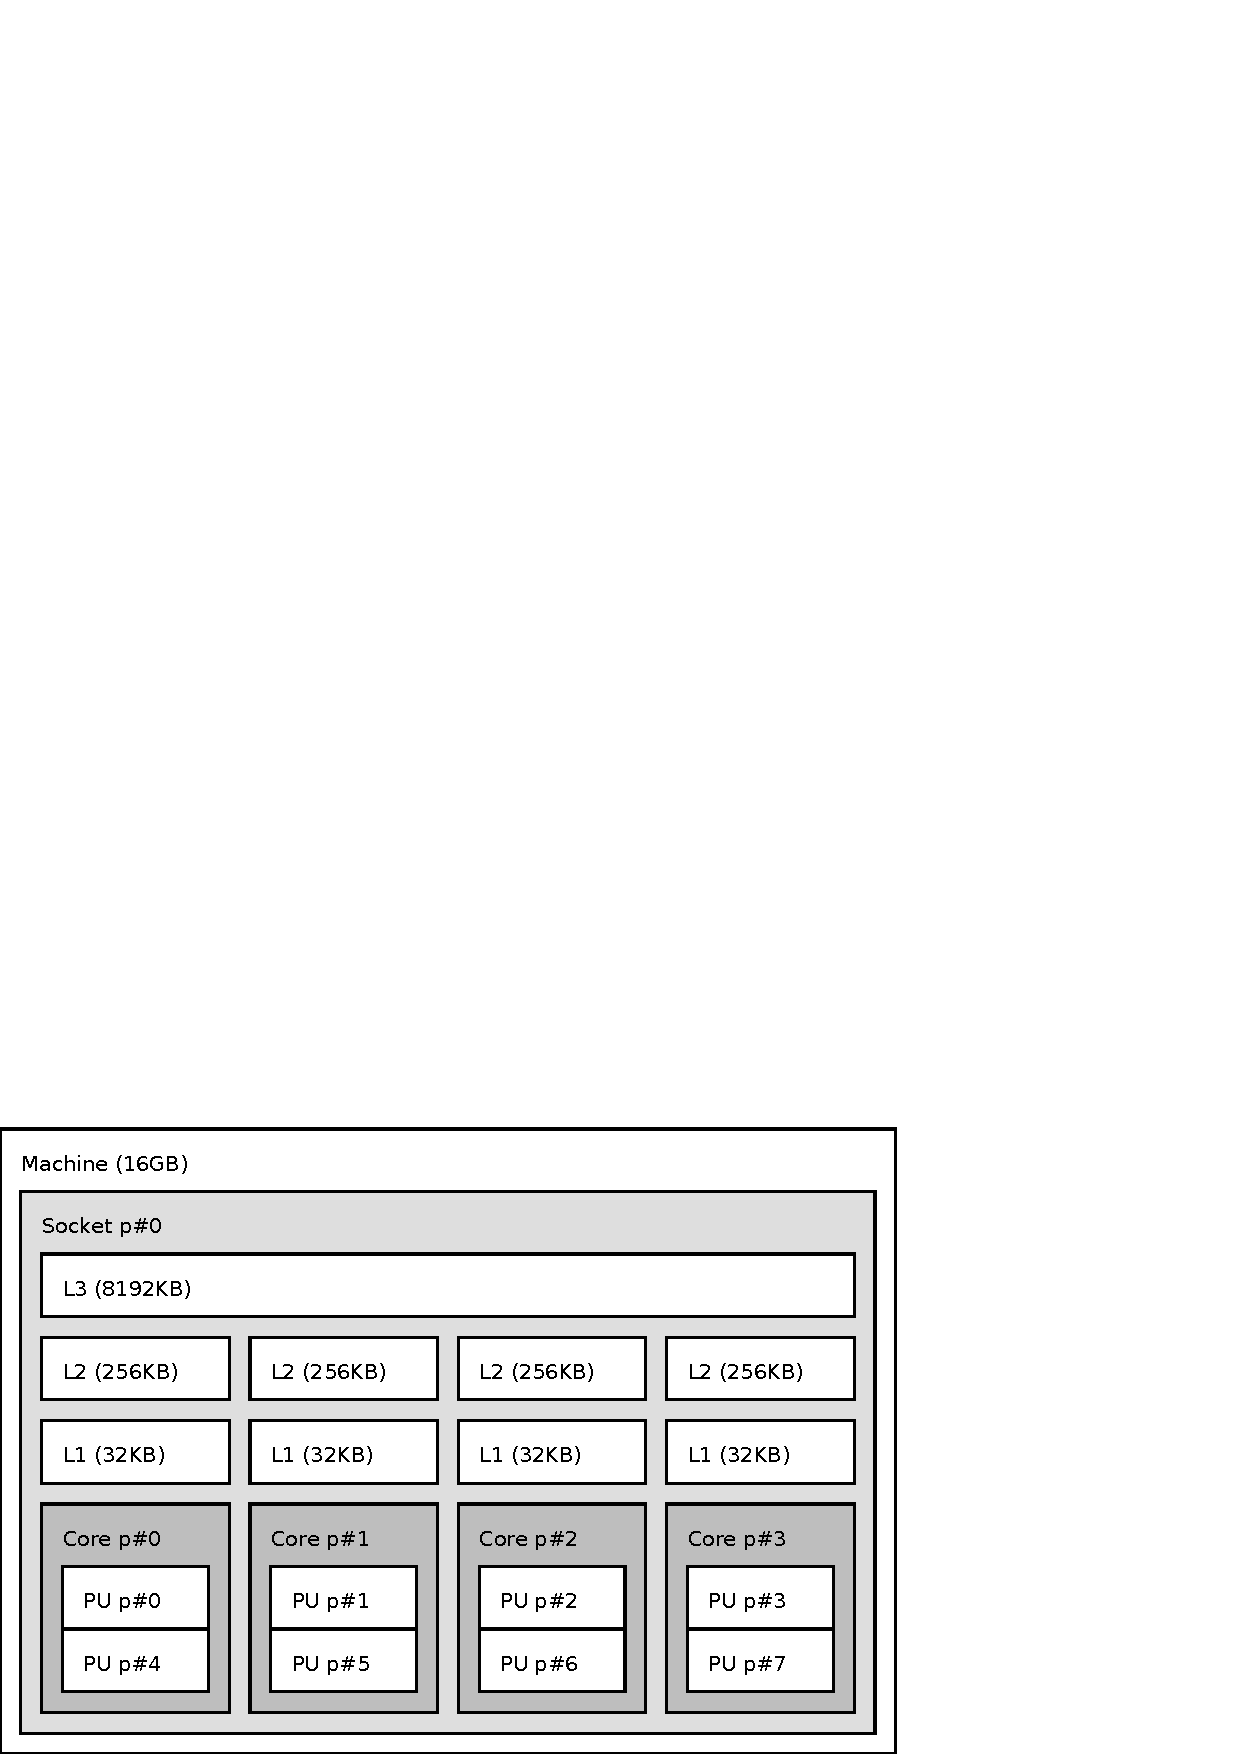
\includegraphics[width=0.75\textwidth]{i7-hierarchy}
\end{center}
\caption{Memory hierarchy of the Intel i7-2600K processor and 16GB of main
memory}
\label{fig:i7_hierarchy}
\end{figure}

\plan{Introduce SMT}
The multi-processor (and multi-core) systems we have been targeting our work
towards have been symmetric multi-processor (SMP) systems.
This means that they have two or more, equivalent processors,
and that the memory is approximately the same distance from each of the
processors (the system is not a non-uniform memory architecture (NUMA)
system).
Many current SMP systems are also symmetric multi-threading (SMT)\footnote{
    Intel commonly calls SMT ``hyper-threading''}
systems.
As an example, figure \ref{fig:i7_hierarchy} shows the memory hierarchy of
an Intel i7-2600K based system with 16GB of memory;
each of the four cores has two hardware threads,
labelled PU (Processing Unit) in the figure.
Each of the four physical processor cores can execute two hardware threads
\emph{concurrently}.
It is important to recognise that hardware threads on the same core are not
executed in parallel;
which is how we are used to thinking of multi-processing.
Instead, each core is able to execute more than one instruction stream at a
time.
If the execution of one instruction stream must wait for something such as a
value to be retrieved from memory,
then the core is able to execute the other instruction stream.
This improves performance by allowing the processor to make use the time
when it would otherwise be stalled.
To allow programs to use SMT systems the the operating system makes the
extra hardware threads available to applications by making it appear as if
the system has more processors than it actually does.
% Allowing each core to run a second thread can increase performance,
% but it will not double it.
When talking about an SMT thread we will say ``hardware thread'',
allowing the term ``thread'' to refer to a software thread managed by the
operating system.

\plan{Explain why we want $P$ engines when there are $P$ processors}
In order to make use of each of the system's processor cores and hardware
threads (``processors'' for brevity)
we should create at least one thread for each processor.
Creating more than this consumes more resources than necessary,
and when more than one thread is actively using the same processor the
operating system must perform context switches between these threads.
Therefore it is best to use exactly one thread per processor,
which is the default.
\plan{Explain briefly how we detect how many processors there are,}
We have been using the
\code{sysconf(\_SC\_NPROCESSORS\_ONLN)}
system call to detect the number of
processors in the system.
On the Intel i7-2600K (figure \ref{fig:i7-hierarchy}
\code{sysconf(\_SC\_NPROCESSORS\_ONLN)}
returns 8.
This is supported on several but not all platforms.
If Mercury cannot detect the number of processors in the system it defaults 
to using a single engine.

\plan{Explain why we want thread pinning.}
We have been relying on the operating system to assign threads onto
processors.
This is usually acceptable,
but it is generally considered more reliable to pin threads to specific
processors.
%This is beginning to become more important as processors are made with
%larger numbers of cores and therefore more complex memory hierarchies.
\plan{Explain how we get thread pinning.}
We can \emph{pin} a thread to a specific processor using the
\code{setcpuaffinity()} system call,
which is available on many Unix-like OSs.
Our initial thread pinning implementation pinned each of Mercury's engines
to a separate processor.
The goals are to ensure that two thread are not contending for the same
processor, leaving another processor idle;
and that threads are not needlessly migrated between processors.
Thread pinning should also work when the user requests fewer engines
than processors.
When the user requests more engines than processors,
only the first $P$ thread are pinned (where there are $P$ processors).

% Benchmarks are inconclusive.
%\begin{table}
%\begin{center}
%\begin{tabular}{rr|r|rrrrrrrr}
%\multicolumn{1}{c|}{Method} &
%\multicolumn{1}{c|}{Pinning} &
%\multicolumn{1}{c|}{Sequmential} &
%\multicolumn{8}{c}{Parallel w/ $N$ Engines} \\
%\Cbr{}& \Cbr{}& \Cbr{TS} & \C{1}& \C{2}& \C{3}& \C{4}& \C{5}& \C{6}&
%    \C{7}& \C{8}\\
%\hline
%\hline
%\multicolumn{11}{c}{Right recursive mandelbrot (max.\ 1024 contexts)} \\
%\hline
%setcpuaffinity() & no
%        & 15.1 & 15.2 & 7.6 & 5.1 & 3.8 & 3.7 & 3.5 & 3.4 & 3.3 \\
%hwloc & no
%        & 15.2 & 15.2 &  7.6 &  5.1 &  3.8 &  3.7 &  3.5 &  3.4 &  3.3 \\
%setcpuaffinity() & yes
%        & -    & 15.2 &  7.6 &  5.1 &  3.8 &  3.7 &  3.6 &  3.4 &  3.3 \\
%hwloc & yes
%        & -    & 15.4 &  7.7 &  5.1 &  3.9 &  3.7 &  3.6 &  3.5 &  3.3 \\
%\end{tabular}
%\end{center}
%\end{table}

\plan{Problem with SMT}


\plan{What about SMT, not all processors are equal.}
This works well on SMP systems that do not use SMT.
On systems that use SMP and SMT
\footnote{
    SMT is sometimes called ``hyper-threading'' especially for marketing.}
(symmetric multi-threading) as well as SMP this causes problems.
Consider the memory hierarchy of the Intel i7-2600K processor
(figure \ref{fig:i7_hierarchy}).
The i7-2600K has four cores, each with two hardware threads,
program units (PUs) in the figure.
If Mercury successfully detects that the system has eight logical processors
or the user specifies eight engines then thread pinning will correctly pin
each engine to a separate thread.
However,
if the user requests only four engines, which cores will be used?
depending on how they are selected,
and how the OS's \code{setcpuaffinity()} system call labels them,
all four Mercury engines could be pinned to just two of the CPU's cores
instead of being distributed uniformly across all four cores.
Uniform distribution will result in higher performance for the Mercury
program,
but it may affect other processes running on the same system.

\plan{How do we handle SMT}
Unfortunately there is no method provided by all operating systems to
determine the system's memory hierarchy.
Therefore we use a third party library
named Portable Hardware Locality (hwloc) \citep{broquedis:2010:hwloc}.
Hwloc provides some tools such as the one that drew figure
\ref{fig:i7_hierarchy},
but more importantly it provides an API for querying the memory hierarchy of
the system and methods for pinning threads to (sets of) cores or hardware
threads.
We use hwloc to determine the number of hardware threads in a system,
and optionally pin engines to hardware threads.
If the user specified the number of engines to use,
then we pin each engine to a hardware thread in each core so that engines
are distributed to cores as evenly as possible.
If the user specifies more engines than are available
(which we admit would be silly) then we allow more than one engine per
hardware thread,
meanwhile keeping engines as evenly distributed as possible amongst the
threads and cores.


%\plan{Further work}
%As we discussed in the previous section,
%knowledge of the memory hierarchy could help make better scheduling
%decisions.
%When using thread pinning we can guarantee that a particular engine is
%running on a particular processor/hardware thread,
%combining this with information about the memory hierarchy such as shared
%caches/sockets we can know which processors share the same cache(s) with the
%current processor either prefer to steal work from them or send work to
%them.



\status{Not written}

\plan{Describe the problem with the current algorithm.}
Engines wake up and periodically check for work by attempting to
steal work,
firstly, this means that there can be up to a 2ms (average 1ms) delay before
a spark is executed.
secondly, this checks for work too often, wasting resources.

\plan{Solution, wake engines for different types of work}
We modified the RTS so that waking an engine is easy, and it can be given a
message so that it knows where to look for work.

\plan{A lot of work went into preventing deadlocks due to race conditions,
a thread that is not yet sleeping if notified must wake up immediately.}

\plan{Extra benefit: when an engine is woken it can be told directly where
to find work, or be given the work directly.}

\plan{Extra benefit: we can be selective about which engine to wake,
while not implemented fully, we can wake a `nearby' engine so that
we can avoid communication between dies or sockets.}

\plan{Show the algorithm for the new idle loop.}
Note that we execute contexts before sparks,
this is more-likely to produce futures and it may reduce memory consumption.

%\subsection{Revised work stealing implementation}

\plan{Work stealing attempts}

\plan{Describe work stealing timeout.}


\plan{Describe problems with associating stacks with contexts}
The number of stacks varies,
Stealing uses a global lock to determine which stack to steal from.

\plan{Prove that even though there are N engines and M contexts and M may be
larger than N, that there will be at most N of the M contexts with work on
their queues}
Therefore:
Stealing is unnecessary complicated.
In pathological cases many attempts can be made without success,
a thief may give up even though there is parallelism.

\plan{We associate stacks with engines}
This removes the above problems how.

\plan{Show stealing algorithm there are any,}
Find out if I started tracking stealing per engine or not.

\plan{Show how this is safe.}
When a parallel conjunction's barrier is executed and a conjunct is
outstanding, if its spark is on this engine's stack it must be at the top of
the stack.
This invariant should be kept because the context can be re-used if
'compatible' work is found at the top of the spark stack.
This invariant is soft.


\begin{table}
\begin{center}
\begin{tabular}{r|rr|rrrr}
\multicolumn{1}{c|}{Version} &
\multicolumn{2}{c|}{Sequmential} &
\multicolumn{4}{c}{Parallel w/ $N$ Engines} \\
\Cbr{} & \C{not TS} & \Cbr{TS} & \C{1}& \C{2}& \C{3}& \C{4}\\
\hline
\hline
\multicolumn{7}{c}{Right recursive mandelbrot (max.\ 1024 contexts)} \\
\hline
Original
& 16.3 (0.93) & 15.2 (1.00)
& 15.5 (0.98) &  7.7 (1.98) &  5.2 (2.92) &  4.1 (3.70) \\
Revised
& 15.3 (1.00) & 15.3 (1.00)
& 15.7 (0.97) &  7.7 (1.98) &  5.3 (2.87) &  3.9 (3.90) \\
\hline
\hline
\multicolumn{7}{c}{Left recursive mandelbrot} \\
\hline
Original
& 15.3 (1.02) & 15.6 (1.00)
& 15.5 (1.00) &  7.6 (2.04) &  5.1 (3.05) &  3.9 (3.95) \\
Revised
& 15.3 (1.02) & 15.7 (0.99)
& 15.8 (0.99) &  7.7 (2.01) &  5.3 (2.94) &  4.0 (3.89) \\
\hline
\hline
\multicolumn{7}{c}{Fibs program (with GC)} \\
\hline
Original
&  3.9 (4.07) & 15.8 (1.00)
& 15.7 (1.00) &  7.7 (2.04) &  5.1 (3.07) &  3.8 (4.12) \\
Revised
&  3.9 (4.04) & 17.0 (0.93)
& 17.0 (0.93) &  8.5 (1.87) &  5.7 (2.76) &  4.3 (3.68) \\
\hline
\hline
\multicolumn{7}{c}{Fibs program (without GC)} \\
\hline
Original
&  3.7 (5.63) & 20.7 (1.00)
& 20.5 (1.01) & 10.1 (2.06) &  6.7 (3.11) &  5.0 (4.11) \\
Revised
&  3.8 (5.44) & 23.2 (0.89)
& 23.2 (0.89) & 11.7 (1.77) &  7.8 (2.65) &  5.9 (3.49) \\
\end{tabular}
\end{center}
\caption{Work stealing results --- revised implementation}
\label{tab:work_stealing_revised}
\end{table}



\plan{Benchmark}


%\section{Proposed scheduling tweaks}
%\label{sec:proposed_tweaks}
%\status{Not written, May move to TS chapter}
%
%I really think that this section will move to the \tscope chapter,
%it will have more in common with that chapter and more data will be
%available.
%Secondly, \tscope can be used with micro-benchmarks to measure the
%average costs of certain operations in the RTS.
%I will not write it until at least the rest of this chapter is finished.

